\newpage\setcounter{dang}{0}
\section{ĐƯỜNG TRÒN TRONG MẶT PHẲNG TỌA ĐỘ}
\subsection{TÓM TẮT LÝ THUYẾT}
\subsubsection{Phương trình đường tròn}
\Opensolutionfile{ans}
\begin{tomtat}
	Đường tròn tâm $I$, bán kính $R$ là tập hợp những điểm $M$ thoả mãn điều kiện $IM=R$.
	\begin{center}
		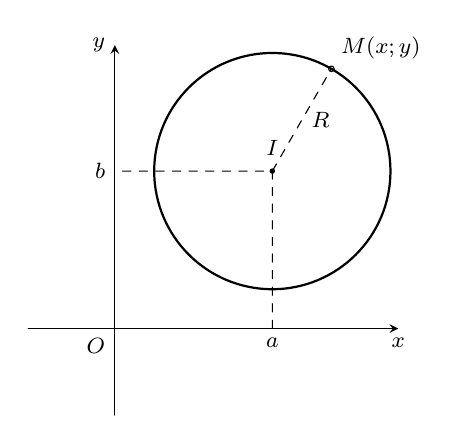
\begin{tikzpicture}[scale=1, font=\footnotesize, line join=round, line cap=round,>=stealth]
			\def\xmin{-1}
			\def\xmax{3.5}
			\def\ymin{-1}
			\def\ymax{3.5}
			\draw[->] (\xmin-0.1,0)--(\xmax+0.1,0) node[below] { $x$};
			\draw[->] (0,\ymin-0.1)--(0,\ymax+0.1) node[left] { $y$};
			\draw (0,0) node [below left] { $O$};
			\path 	(2,2) coordinate (I) (4,0)
					(2,2) arc (180:120:1.5cm) coordinate (M);
			\draw[dashed] (2,0)--(I)--(0,2) (I)--(M) node[pos=0.5,right] {$R$};
			\draw[thick] (2,2) circle (1.5cm);
			\draw 	(M) circle (1pt) node[above right] {$M(x;y)$}
					(2,0) node[below] {$a$}
					(0,2) node[left] {$b$}; 
			\foreach \p/\g in {I/90} \fill[black] (\p) circle(1pt)+(\g:0.3) node{$\p$};
		\end{tikzpicture}
	\end{center}
	\begin{dn}
		Trong mặt phẳng $Oxy$, điểm $M(x;y)$ thuộc đường tròn $(C)$, tâm $I(a;b)$, bán kính $R$ khi và chỉ khi
		\begin{align}
			\left(x-a\right)^2+\left(y-b\right)^2=R^2. \tag{1} \label{0H3-1-1}
		\end{align}
	Ta gọi \eqref{0H3-1-1} là phương trình của đường tròn $(C)$.
	\end{dn}

	\begin{vd}\hfill%[DA TexBook 10,Họa Sĩ Sân Cỏ]%[0H3Y2-1]
		\begin{enumerate}
			\item Tìm tâm và bán kính của đường tròn $(C)$ có phương trình $(x+1)^2 + (y-2)^2=3$.
			\item Viết phương trình đường tròn $(C')$ có tâm $I'(2;0)$ và có bán kính bằng $\sqrt{3}$ lần bán kính đường tròn $(C)$.
		\end{enumerate}
		\loigiai{
			\begin{enumerate}
				\item Ta viết phương trình đường tròn $(C)$ dưới dạng $$\left(x-(-1)\right)^2 + \left(y-2\right)^2=\left(\sqrt{3}\right)^2.$$
				Vậy $(C)$ có tâm $I(-1;2)$ và bán kính $R=\sqrt{3}$.
				\item Đường tròn $(C')$ có tâm $I'(2;0)$ và có bán kính $R'=\sqrt{3} \cdot R= 3$ nên có phương trình
				$$\left(x-2\right)^2 + y^2=9.$$
			\end{enumerate}
		}
	\end{vd}
	\begin{nx}
		Phương trình \eqref{0H3-1-1} tương đương với 
		$$x^2+y^2-2ax-2by+\left(a^2+b^2-R^2\right)=0.$$
	\end{nx}
	\begin{vd}%[DA TexBook 10,Họa Sĩ Sân Cỏ]%[0H3K2-1]
		Cho $a,b,c$ là các hằng số. Tìm tập hợp những điểm $M(x;y)$ thoả mãn phương trình
		\begin{align}
			x^2+y^2-2ax-2by+c=0. \tag{2} \label{0H3-1-2}
		\end{align}
	\end{vd}
	\loigiai{
		Phương trình \eqref{0H3-1-2} tương đương với
		$$\left(x-a\right)^2+\left(y-b\right)^2+c-a^2-b^2=0 \Leftrightarrow \left(x-a\right)^2+\left(y-b\right)^2=a^2+b^2-c.$$
		Xét $I(a;b)$, khi đó, $IM=\sqrt{\left(x-a\right)^2+\left(y-b\right)^2}$ và phương trình trên trở thành
		\begin{align}
			IM^2=a^2+b^2-c. \tag{3} \label{0H3-1-3}
		\end{align}
	Từ đó, ta xét các trường hợp sau:
	\begin{itemize}
		\item Nếu $a^2+b^2-c>0$ thì tập hợp những điểm $M$ thoả mãn \eqref{0H3-1-2} là đường tròn tâm $I(a;b)$, bán kính $R=\sqrt{a^2+b^2-c}$.
		\item Nếu $a^2+b^2-c=0$ thì \eqref{0H3-1-3} $\Leftrightarrow IM=0$. Do đó, tập hợp những điểm $M$ thoả mãn \eqref{0H3-1-2} chỉ gồm một điểm là $I(a;b)$.
		\item  Nếu $a^2+b^2-c<0$ thì tập hợp những điểm $M$ là tập rỗng.
	\end{itemize}
	}
	\begin{note}
		Phương trình $x^2+y^2-2ax-2by+c=0$ là phương trình của một đường tròn $(C)$ khi và chỉ khi $a^2+b^2-c>0$. Khi đó, $(C)$ có tâm $I(a;b)$ và bán kính $R=\sqrt{a^2+b^2-c}$.
	\end{note}
	\begin{vd}%[DA TexBook 10,Họa Sĩ Sân Cỏ]%[0H3Y2-1]
		Xét xem các phương trình sau có là phương trình của đường tròn không? Hãy xác định tâm và bán kính của các đường tròn đó (nếu có).
		\begin{enumerate}
			\item $x^2+y^2+2x-6y-15=0.$ \quad(1)
			\item $2x^2+2y^2+4x+8y+14=0.$ \quad(2)
		\end{enumerate}
		\loigiai{
			\begin{enumerate}
				\item Ta có $\heva{
					-2a&=2 \\ 
					-2b&=-6 \\ 
					c&=-15 \\ 
				}\Rightarrow \heva{
					& a=-1 \\ 
					& b=3 \\ 
					& c=-15 \\ 
				}\Rightarrow a^2+b^2-c=25 > 0$. \\
				Vậy phương trình (1) là phương trình của đường tròn $(C)$ có tâm $I\left(-1;\ 3\right)$ và bán kính $R=5$.
				\item $(2)\Leftrightarrow x^2+y^2+2x+4y+7=0$.\\ Ta có $\heva{
					-2a&=2 \\ 
					-2b&=4 \\ 
					  c&=7 \\ 
				}\Rightarrow \heva{
					& a=-1 \\ 
					& b=-2 \\ 
					& c=7 \\ 
				}\Rightarrow a^2+b^2-c=-2 < 0$. \\
				Vậy phương trình (2) không là phương trình của đường tròn.
			\end{enumerate}
		}
	\end{vd}
	\begin{vd}%[DA TexBook 10,Họa Sĩ Sân Cỏ]%[0H3B2-2]
		Lập phương trình đường tròn đi qua ba điểm $A\left(-2;4\right),B\left(5;5\right),C\left(6;-2\right)$.
		\loigiai{
			\begin{itemize}
				\item \textit{Cách 1.} Các đoạn thẳng $AB,AC$ tương ứng có trung điểm là $M\left(\dfrac{3}{2};\dfrac{9}{2}\right), N\left(2;1\right)$. Đường thẳng trung trực $\Delta_{1}$ của đoạn thẳng $AB$ đi qua $M\left(\dfrac{3}{2};\dfrac{9}{2}\right)$ và có vectơ pháp tuyến $\vec{AB}=\left(7;1\right)$ nên phương trình của đường thẳng $\Delta_{1}$ là
				$$7\left(x-\dfrac{3}{2}\right)+1\left(y-\dfrac{9}{2}\right)=0\,\,\text{hay}\,\,7x+y-15=0.$$
				Đường thẳng trung trực $\Delta_{2}$ của đoạn thẳng $AC$ đi qua $N\left(2;1\right)$ và có vectơ pháp tuyến $\vec{AC}=\left(8;-6\right)$.\\
				Vì $\vec{AC}=\left(8;-6\right)$ cùng phương với $\vec{n_2}=\left(4;-3\right)$ nên phương trình của đường thẳng $\Delta_{2}$ là
				$$4\left(x-2\right)-3\left(y-1\right)=0\,\,\text{hay}\,\,4x-3y-5=0.$$
				Tâm $I$ của đường tròn $(C)$ cách đều ba điểm $A,B,C$ nên $I$ là giao điểm của $\Delta_{1}$ và $\Delta_{2}$\\
				Vậy toạ độ điểm $I$ là nghiệm của hệ phương trình $$\heva{&7x+y-15=0\\&4x-3y-5=0} \Leftrightarrow \heva{&x=2\\&y=1.}$$
				Suy ra $I(2;1)$. Đường tròn $(C)$ có bán kính $IA=5$.\\ Vậy phương trình đường tròn $(C)$ là $$(C):(x-2)^2+(y-1)^2=25.$$
				\item \textit{Cách 2.} Gọi phương trình đường tròn (C) có dạng là: $x^2+y^2-2ax-2by+c=0 $.\\
				Do đường tròn đi qua ba điểm $A,B,C$ nên ta có hệ phương trình
				\begin{align*}
					\heva{
						A\left(-2;4\right) &\in (C)\\
						B\left(5;5\right) &\in (C)\\
						C\left(6;-2\right) &\in (C)}
					\Leftrightarrow \heva{
						4+16+4a-8b+c&=0 \\ 
						25+25-10a-10b+c&=0 \\ 
						36+4-12a+4b+c&=0}
					\Leftrightarrow \heva{
						& a=2 \\ 
						& b=1 \\ 
						& c=-20.}
				\end{align*} 
				Vậy phương trình đường tròn cần tìm là $x^2+y^2-4x-2y-20=0 $.
				\item \textit{Cách 3.} Gọi $I\left(x;y\right)$ và $R$ là tâm và bán kính đường tròn cần tìm. Ta suy ra:
				\begin{align*}
					IA=IB=IC \Leftrightarrow \heva{
						&IA^2=IB^2 \\
						&IA^2=IC^2.}
				\end{align*}
				nên ta có hệ 
				\begin{align*}
					\heva{
						&(x+2)^2+(y-4)^2=(x-5)^2+(y-5)^2 \\
						&(x+2)^2+(y-4)^2=(x-6)^2+(y+2)^2}
					\Leftrightarrow \heva{& x=2 \\
						& y=1.}
				\end{align*}
				Suy ra $I(2; 1)$, bán kính $IA=5$.\\
				Vậy phương trình đường tròn cần tìm $(C):(x-2)^2+(y-1)^2=25$.
			\end{itemize}
		}
	\end{vd}
\subsubsection{Phương trình tiếp tuyến đường tròn}
	\begin{dn}
		Cho điểm $M\left(x_0;y_0\right)$ thuộc đường tròn $(C) \colon \left(x-a\right)^2+\left(y-b\right)^2=R^2$ (tâm $I(a;b)$, bán kính $R$). Khi đó, tiếp tuyến $\Delta$ của $(C)$ tại $M\left(x_0;y_0\right)$ có vectơ pháp tuyến $\vec{MI}=\left(a-x_0;b-y_0\right)$ và phương trình $$\left(a-x_0\right)\left(x-x_0\right)+\left(b-y_0\right)\left(y-y_0\right)=0.$$
		\begin{center}
			\begin{tikzpicture}[scale=1, font=\footnotesize, line join=round, line cap=round,>=stealth]
				\def\xmin{-1}
				\def\xmax{3.5}
				\def\ymin{-1}
				\def\ymax{3.5}
				\pgfmathsetmacro\r{sqrt(2)}
				\path 	(0,0) coordinate (I)
						(-0.5,2.5) coordinate (A)
						(3,-1) coordinate (B);
				\draw[thick,name path=tr] (0,0) circle (\r);
				\draw[thick,name path=th] (A)--(B) node[above right] {$\Delta$}; 
				\path[name intersections={of=tr and th}] (intersection-1) coordinate (M);
				\draw (I)--(M);
				\foreach \p/\g in {I/90,M/45} \fill[black] (\p) circle(1pt)+(\g:0.3) node{$\p$};
				\draw 	pic[draw,angle radius=2mm]{right angle=A--M--I};
			\end{tikzpicture}
		\end{center}
	\end{dn}
	\begin{vd}%[DA TexBook 10,Họa Sĩ Sân Cỏ]%[0H3Y2-3]
		Viết phương trình tiếp tuyến của đường tròn $(C): (x-2)^2+(y+3)^2=5$ tại điểm $M(3;-1)$.
		\loigiai{
			Đường tròn $(C)$ có tâm $I(2;-3)$.\\
			Phương trình tiếp tuyến của $(C)$ tại điểm $M(3;-1)$ là 
			\begin{align*}
				&(3-2)(x-3)+(-1+3)(y+1)=0 \\ \Leftrightarrow\, &x+2y-1=0.
			\end{align*}
			Vậy phương trình  tiếp tuyến của $(C)$ tại điểm $M(3;-1)$ là $ x+2y-1=0 $.
		}
	\end{vd}
	\begin{vd}%[DA TexBook 10,Họa Sĩ Sân Cỏ]%[0H3Y2-3]
		Viết phương trình tiếp tuyến của đường tròn $(C):x^2+y^2-2x=0$ tại điểm $M(1;1)$.
		\loigiai{
			Đường tròn $(C)$ có tâm $I(1;0)$.\\
			Phương trình tiếp tuyến của $(C)$ tại điểm $M(1;1)$ là
			\begin{align*}
				&(1-1)(x-1)+(0+1)(y-1)=0 \\ \Leftrightarrow\, &y=1.
			\end{align*}
		}
	\end{vd}
\end{tomtat}
\subsection{CÁC DẠNG TOÁN THƯỜNG GẶP}
\begin{dang}{Tìm tâm và bán kính đường tròn.}
	\textbf{\textit{Phương pháp giải.}}
	\begin{itemize}
		\item \textit{Cách 1.} Đưa phương trình về dạng $(C)\colon x^2+y^2-2ax-2by+c=0$.\qquad (1) 
		\begin{enumerate}[-]
			\item Nếu $a^2+b^2-c>0$ thì (1) là phương trình đường tròn $(C)$ có tâm $I\left(a;b\right)$ và bán kính $R=\sqrt{a^2+b^2-c}$.
			\item Nếu $a^2+b^2-c\le 0$ thì (1) không phải là phương trình đường tròn.
		\end{enumerate}
		\item \textit{Cách 2.} Đưa phương trình về dạng $(x-a)^2+(y-b)^2=m$.\qquad (2)
		\begin{enumerate}[-]
			\item Nếu $m > 0$ thì (2) là phương trình đường tròn có tâm $I\left(a;b\right)$ và bán kính $R=\sqrt{m}$.
			\item Nếu $m\le 0$ thì (2) không phải là phương trình đường tròn.
		\end{enumerate}
	\end{itemize}
\end{dang}
\begin{vd}%[Du an tex sach 10-2022]%[0H3Y2]
	Xét xem các phương trình sau có là phương trình của đường tròn không? Hãy xác định tâm và bán kính của các đường tròn đó (nếu có).
	\begin{enumerate}
		\item $x^2+y^2+2x-4y+9=0$. \qquad(1)
		\item $x^2+y^2-6x+4y+13=0$. \qquad(2)
		\item $2x^2+2y^2-6x-4y-1=0$. \qquad(3)
		\item $2x^2+y^2+2x-3y+9=0$. \qquad(4)
	\end{enumerate}
	\loigiai{
		\begin{enumerate}
			\item Phương trình (1) có dạng $x^2+y^2-2ax-2by+c=0 $ với $a=-1;b=2;c=9$.\\ 
			Ta có $a^2+b^2-c=1+4-9 < 0$.\\
			Vậy phương trình (1) không phải là phương trình đường tròn.
			\item Ta có  $a^2+b^2-c=9+4-13=0$.\\
			Suy ra phương trình (2) không phải là phương trình đường tròn.
			\item Ta có  $(3)\Leftrightarrow x^2+y^2-3x-2y-\dfrac{1}{2}=0\Leftrightarrow \left(x-\dfrac{3}{2}\right)^{2}+(y-1)^2=\dfrac{15}{4}$.\\
			Vậy phương trình (3) là phương trình đường tròn tâm $I\left(\dfrac{3}{2};1\right)$ bán kính $R=\dfrac{\sqrt{15}}{2}$.
			\item Phương trình (4) không phải là phương trình đường tròn vì hệ số của $x^2$ và $y^2$ khác nhau.
		\end{enumerate}
	}
\end{vd}
\begin{vd}%[Du an tex sach 10-2022]%[0H3B2]
	Cho phương trình $~x^2+y^2-2mx-4(m-2)y+6-m=0$. \qquad(1)\\ Tìm điều kiện của $m$ để $(1)$ là phương trình đường tròn.
	\loigiai{
		Ta có $a=m$, $b=2(m-2)$, $c=6-m$.\\
		Phương trình (1) là phương trình đường tròn khi và chỉ khi $a^2+b^2-c > 0$.\\
		Hay $m^2+4(m-2)^2-6+m > 0\Leftrightarrow 5m^2-15m+10 > 0\Leftrightarrow \hoac{
			& m > 2 \\ 
			& m < 1.}$
	}
\end{vd}
\begin{dang}{Viết phương trình đường tròn.}
	\textbf{\textit{Phương pháp giải.
	}}
	\begin{itemize}
		\item \textit{Cách 1.} 
		\begin{enumerate}[-]
			\item Tìm tọa độ tâm $I\left(a;b\right)$ của đường tròn $(C)$.
			\item Tìm bán kính $R$ của đường tròn $(C)$.
			\item Viết phương trình của $(C)$ theo dạng $(x-a)^2+(y-b)^2=R^2$.
		\end{enumerate}
		\item \textit{Cách 2.} 
		\begin{enumerate}[-]
			\item Giả sử phương trình đường tròn $(C)$ là  $x^2+y^2-2ax-2by+c=0$ (hoặc $x^2+y^2+2ax+2by+c=0 $) ($a^2+b^2-c>0$).
			\item Từ điều kiện của đề bài thiết lập hệ phương trình với ba ẩn là $a,\,b,\,c$.
			\item Giải hệ để tìm $a,\,b,\,c$, từ đó tìm được phương trình đường tròn $(C)$.
		\end{enumerate}
	\end{itemize}
	\textbf{\textit{Chú ý.}}
	\begin{itemize}
		\item Cho đường tròn $(C)$ có tâm $I$ và bán kính $R$.
		$A\in (C)\Leftrightarrow IA=R$.
		\item $(C)$ tiếp xúc với đường thẳng $\Delta $ tại $A\Leftrightarrow IA=\mathrm{d}\left(I;\Delta\right)=R$.
		\item $(C)$ tiếp xúc với hai đường thẳng ${\Delta}_1$ và ${\Delta}_2\Leftrightarrow \mathrm{d}\left(I;{\Delta}_1\right)=\mathrm{d}\left(I;{\Delta}_2\right)=R$.
		\item $(C)$ cắt đường thẳng ${\Delta}_3$ theo dây cung có độ dài $a \Leftrightarrow \left(\mathrm{d}\left(I;{\Delta}_3\right)\right)^2+\dfrac{a^2}{4}=R^2$.
	\end{itemize}
\end{dang}
\begin{vd}%[Du an tex sach 10-2022]%[0H3Y2]
	Viết phương trình đường tròn có tâm $I(3;-5)$ bán kính $R=2$.
	\loigiai{
		Ta có phương trình đường tròn là 
		$(x-3)^2+(y+5)^2=2^2\Leftrightarrow x^2+y^2-6x+10y+30=0$.
	}
\end{vd}
\begin{vd}%[Du an tex sach 10-2022]%[0H3Y2]
	Viết phương trình đường tròn đường kính $AB$ với $A\left(1;6\right),B\left(-3;2\right)$.
	\loigiai{
		Đường tròn đường kính $AB$ có
		\begin{itemize}
			\item Tâm $I\left(-1;4\right)$ là trung điểm $AB$.
			\item Bán kính $R=\dfrac{AB}{2}=2\sqrt{2}$.
		\end{itemize}
		Do đó phương trình đường tròn là \\ $(x+1)^2+(y-4)^2=\left(2\sqrt{2}\right)^2\Leftrightarrow x^2+y^2+2x-8y+9=0$.
	}
\end{vd}
\begin{vd}%[Du an tex sach 10-2022]%[0H3Y2]
	Viết phương trình đường tròn $(C)$ có tâm $I\left(-1;2\right)$ và tiếp xúc với đường thẳng $\Delta \colon x-2y+7=0$.
	\loigiai{
		Bán kính đường tròn $(C)$ chính là khoảng cách từ $I$ tới đường thẳng $\Delta $ nên
		\begin{align*}
			R=\mathrm{d}\left(I;\Delta\right)=\dfrac{\left|-1-4+7\right|}{\sqrt{1+4}}=\dfrac{2}{\sqrt{5}}.
		\end{align*}
		Vậy phương trình đường tròn $(C)$ là  $(x+1)^2+(y-2)^2=\dfrac{4}{5}$.
	}
\end{vd}
\begin{vd}%[Du an tex sach 10-2022]%[0H3Y2]
	Viết phương trình đường tròn tâm $I\left(-2;1\right)$, cắt đường thẳng $\Delta \colon x-2y+3=0$ tại hai điểm $A,B$ thỏa mãn $AB=2$.
	\loigiai{
		Gọi $h$ là khoảng cách từ $I$ đến đường thẳng $\Delta $. Ta có
		\begin{align*}
			h=\mathrm{d}\left(I,\Delta\right)=\dfrac{\left|-2-2+3\right|}{\sqrt{1^2+\left(-2\right)^{2}}}=\dfrac{1}{\sqrt{5}}.
		\end{align*} 
		Gọi $R$ là bán kính đường tròn, từ giả thiết suy ra
		
		\begin{align*}
			R=\sqrt{h^2+\dfrac{AB^2}{4}}=\sqrt{\dfrac{1}{5}+\dfrac{2^2}{4}}=\sqrt{\dfrac{6}{5}}.
		\end{align*}
		Vậy phương trình đường tròn là  $(x+2)^2+(y-1)^2=\dfrac{6}{5}$.
	}
\end{vd}
\begin{vd}%[Du an tex sach 10-2022]%[0H3B2]
	Viết phương trình đường tròn đi qua ba điểm $M\left(-2;4\right),\,N\left(5;5\right),\,P\left(6;-2\right)$.
	\loigiai{
		\begin{itemize}
			\item \textit{Cách 1.} Gọi phương trình đường tròn (C) có dạng là  $x^2+y^2-2ax-2by+c=0$.\\
			Do đường tròn đi qua ba điểm $M,N,P$ nên ta có hệ phương trình
			$$\heva{&
				4+16+4a-8b+c=0 \\& 
				25+25-10a-10b+c=0 \\ &
				36+4-12a+4b+c=0}
			\Leftrightarrow \heva{
				& a=2 \\ 
				& b=1 \\ 
				& c=-20.}$$		
			Vậy phương trình đường tròn cần tìm là  $x^2+y^2-4x-2y-20=0$.
			\item \textit{Cách 2.} Gọi $I\left(x;y\right)$ và $R$ là tâm và bán kính đường tròn cần tìm. Ta suy ra
			\begin{align*}
				IM=IN=IP \Leftrightarrow \heva{
					&IM^2=IN^2 \\
					&IM^2=IP^2.}
			\end{align*}
			nên ta có hệ 
			\begin{align*}
				\heva{
					&(x+2)^2+(y-4)^2=(x-5)^2+(y-5)^2 \\
					&(x+2)^2+(y-4)^2=(x-6)^2+(y+2)^2}
				\Leftrightarrow \heva{& x=2 \\
					& y=1.}
			\end{align*}
			Suy ra $I(2; 1)$, bán kính $IA=5$.\\
			Vậy phương trình đường tròn cần tìm $(C)\colon (x-2)^2+(y-1)^2=25$.
		\end{itemize}
	}
\end{vd}
\begin{vd}%[Du an tex sach 10-2022]%[0H3K2]
	Cho hai điểm $A\left(8;0\right)$ và $B\left(0;6\right)$.
	\begin{enumerate}
		\item Viết phương trình đường tròn ngoại tiếp tam giác $OAB$.
		\item Viết phương trình đường tròn nội tiếp tam giác $OAB$.
	\end{enumerate}
	\loigiai{
		\begin{enumerate}
			\item Ta có tam giác $OAB$ vuông ở $O$ nên tâm $I$ của đường tròn ngoại tiếp tam giác là trung điểm của cạnh huyền $AB$ suy ra $I\left(4;3\right)$ và bán kính $$R=IA=\sqrt{(8-4)^2+(0-3)^2}=5.$$
			Vậy phương trình đường tròn ngoại tiếp tam giác $OAB$ là  $ (x-4)^2+(y-3)^2=25$.
			\item Ta có $OA=8;OB=6;AB=\sqrt{8^2+6^2}=10$.\\
			Mặt khác $\dfrac{1}{2}OA\cdot OB=pr$ (vì cùng bằng diện tích tam giác $ABC$).\\
			Suy ra $r=\dfrac{OA\cdot OB}{OA+OB+AB}=2$.\\
			Dễ thấy đường tròn cần tìm có tâm thuộc góc phần tư thứ nhất và tiếp xúc với hai trục tọa độ nên tâm của đường tròn có tọa độ là $\left(2;2\right)$.\\
			Vậy phương trình đường tròn nội tiếp tam giác $OAB$ là $(x-2)^2+(y-2)^2=4$.
		\end{enumerate}
	}
\end{vd}
\begin{vd}%[Du an tex sach 10-2022]%[0H3K2]
	Trong mặt phẳng với hệ tọa độ $Oxy$, cho đường thẳng $d\colon 2x-y-5=0$ và hai điểm $A\left(1;2\right), B\left(4;1\right)$. Viết phương trình đường tròn $(C)$ có tâm thuộc $d$ và đi qua hai điểm $A, B$.
	\loigiai{
		\immini{
			\begin{itemize}
				
				\item \textit{Cách 1.} Gọi $I$ là tâm của $(C)$. Do $I\in d$ nên $I\left(t;2t-5\right)$.\\
				Hai điểm $A, B$ cùng thuộc $(C)$ nên 
				\begin{align*}
					IA=IB & \Leftrightarrow (1-t)^2+\left(7-2t\right)^2=(4-t)^2+\left(6-2t\right)^2\\
					& \Leftrightarrow t=1.
				\end{align*}
				Suy ra $I(1;-3)$ và bán kính $R=IA=5$.\\
				Vậy phương trình đường tròn cần tìm là 
				\begin{align*}
					(C)\colon (x-1)^2+(y+3)^2=25.
				\end{align*}
			\end{itemize}
		}
		{
			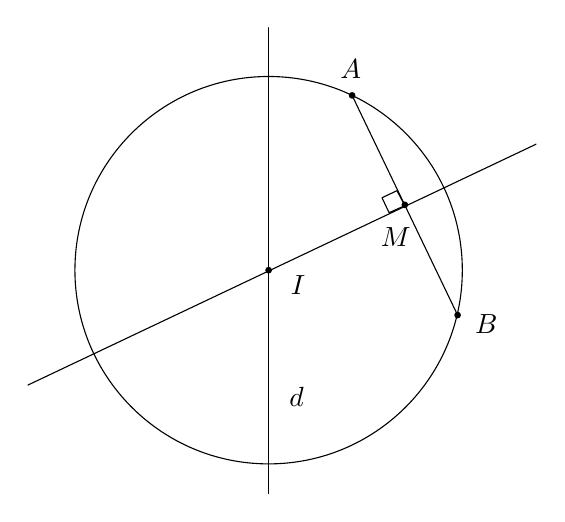
\begin{tikzpicture}[line cap=round,line join=round,>=stealth,x=1.0cm,y=1.0cm]
				\clip(1.24,-1.) rectangle (7.7,4.92);
				\draw (5.93,2.85) -- (5.74,2.76) -- (5.83,2.57) -- (6.03,2.66) -- cycle; 
				\draw (4.3,1.84) circle (2.46cm);
				\draw (5.36,4.06)-- (6.7,1.27);
				\draw [domain=1.24:7.7] plot(\x,{(-0.36--0.82*\x)/1.73});
				\draw (4.3,-1.) -- (4.3,4.92);
				\draw (5.6,4.4) node[left] {$A$};
				\draw (6.8,1.4) node[anchor=north west] {$B$};
				\draw (5.6,2.5) node[anchor=north west] {$M$};
				\draw (4.44,0.48) node[anchor=north west] {$d$};
				\draw (4.46,1.9) node[anchor=north west] {$I$};
				\draw [fill=black] (4.3,1.84) circle (1.0pt);
				\draw [fill=black] (5.36,4.06) circle (1.0pt);
				\draw [fill=black] (6.7,1.27) circle (1.0pt);
				\draw [fill=black] (6.03,2.67) circle (1.0pt);
			\end{tikzpicture}
		}
		\begin{itemize}
			\item \textit{Cách 2. }Gọi $M\left(\dfrac{5}{2};\dfrac{3}{2}\right)$ là trung điểm $AB$. Đường trung trực của đoạn $AB$ đi qua $M$ và nhận $\vec{AB}=(3;-1)$ làm vectơ pháp tuyến nên có phương trình $\Delta \colon 3x-y-6=0$.\\
			Tọa độ tâm $I$ của $(C)$ là nghiệm của hệ $\heva{
				& 2x-y-5=0 \\ 
				& 3x-y-6=0 
			}\Rightarrow I(1;-3)$.\\
			Bán kính của đường tròn bằng $R=IA=5$.\\
			Vậy phương trình đường tròn cần tìm $(C)\colon (x-1)^2+(y+3)^2=25$.
		\end{itemize}
	}
\end{vd}
\begin{vd}%[Du an tex sach 10-2022]%[0H3K2]
	Trong mặt phẳng với hệ tọa độ $Oxy$, cho hai đường thẳng $d_1\colon x+3y+8=0$, $d_2\colon 3x-4y+10=0$ và điểm $A\left(-2;1\right)$. Viết phương trình đường tròn $(C)$ có tâm thuộc $d_1$, đi qua điểm $A$ và tiếp xúc với $d_2$.
	\loigiai{
		\immini{
			Gọi $I$ là tâm của $(C)$. Do $I\in d_1$ nên $I\left(-3t-8;t\right)$.\\
			Theo giả thiết bài toán, ta có 
			\begin{align*}
				\mathrm{d}\left(I,d_2\right)=IA & \Leftrightarrow \dfrac{\left| 3\left(-3t-8\right)-4t+10\right|}{\sqrt{3^2+4^2}}=\sqrt{\left(-3t-8+2\right)^2+(t-1)^2} \\ 
				&\Leftrightarrow t=-3. 
			\end{align*}
			
			Suy ra $I(1;-3)$ và bán kính $R=IA=5$.\\
			Vậy phương trình đường tròn cần tìm là
			\begin{align*}
				(C)\colon (x-1)^2+(y+3)^2=25.
			\end{align*}
		}
		{
			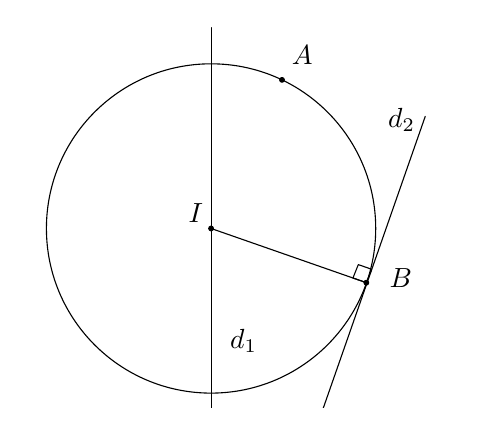
\begin{tikzpicture}[line cap=round,line join=round,>=stealth,x=1.0cm,y=1.0cm,scale=.85]
				\clip(1.56,-0.84) rectangle (7.94,4.84);
				\draw[fill opacity=0.1] (6.7,1.23) -- (6.5,1.3) -- (6.42,1.1) -- (6.62,1.03) -- cycle; 
				\draw (4.3,1.84) circle (2.46cm);
				\draw (4.3,-0.84) -- (4.3,4.84);
				\draw (5.36,4.72) node[anchor=north west] {$A$};
				\draw (6.82,1.38) node[anchor=north west] {$B$};
				\draw (4.44,0.48) node[anchor=north west] {$d_1$};
				\draw (3.82,2.36) node[anchor=north west] {$I$};
				\draw (4.3,1.84)-- (6.62,1.03);
				\draw [domain=1.5:7.5] plot(\x,{(-14.55--2.32*\x)/0.811});
				\draw (6.8,3.78) node[anchor=north west] {$d_2$};
				\draw [fill=black] (4.3,1.84) circle (1.0pt);
				\draw [fill=black] (5.36,4.06) circle (1.0pt);
				\draw [fill=black] (6.62,1.03) circle (1.0pt);
			\end{tikzpicture}
		}
	}
\end{vd}
\begin{vd}%[Du an tex sach 10-2022]%[0H3G2]
	Viết phương trình đường tròn $(C)$ có tâm nằm trên đường thẳng $d \colon x-6y-10=0$ và tiếp xúc với hai đường thẳng có phương trình $d_1\colon 3x+4y+5=0$ và $d_2\colon 4x-3y-5=0$.
	\loigiai{
		\immini{
			Vì đường tròn cần tìm có tâm $K$ nằm trên đường thẳng d nên gọi $K\left(6a+10;a\right)$
			Mặt khác đường tròn tiếp xúc với $d_1,d_2$ nên khoảng cách từ tâm $K$ đến hai đường thẳng này bằng nhau và bằng bán kính $R$ suy ra
			\allowdisplaybreaks
			\begin{eqnarray*}
				&& \dfrac{\left| 3(6a+10)+4a+5\right|}{5}=\dfrac{\left| 4(6a+10)-3a-5\right|}{5} \\ 
				& \Leftrightarrow& \left| 22a+35\right|=\left| 21a+35\right| \\ 
				& \Leftrightarrow& \hoac{
					& a=0 \\ 
					& a=\dfrac{-70}{43}.}
			\end{eqnarray*}
		}
		{
			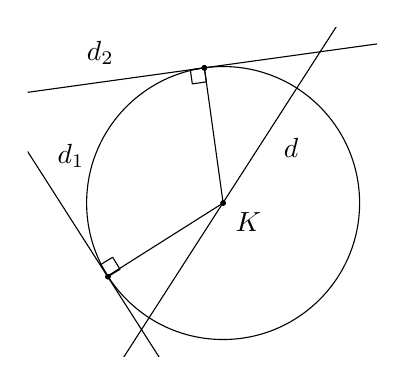
\begin{tikzpicture}[line cap=round,line join=round,>=stealth,x=1.0cm,y=1.0cm,scale=.85]
				\clip(1.32,-1.26) rectangle (6.54,3.66);
				\draw[fill opacity=0.1] (3.75,3.03) -- (3.78,2.82) -- (3.99,2.85) -- (3.96,3.06) -- cycle; 
				\draw[fill opacity=0.1] (2.7,0.05) -- (2.59,0.23) -- (2.41,0.12) -- (2.52,-0.06) -- cycle; 
				\draw (4.24,1.04) circle (2.0393136100168605cm);
				\draw (4.24,1.04)-- (3.96,3.06);
				\draw [domain=1.32:6.54] plot(\x,{(-5.0724-0.28*\x)/-2.02});
				\draw (4.24,1.04)-- (2.5,-0.06);
				\draw [domain=1.32:6.54] plot(\x,{(--4.26-1.72*\x)/1.1});
				\draw [,domain=1.32:6.54] plot(\x,{(-13.2--3.7*\x)/2.38});
				\draw (4.28,1.04) node[anchor=north west] {$K$};
				\draw (5.,2.16) node[anchor=north west] {$d$};
				\draw (1.62,2.06) node[anchor=north west] {$d_1$};
				\draw (2.06,3.6) node[anchor=north west] {$d_2$};
				\draw [fill=black] (4.24,1.04) circle (1.0pt);
				\draw [fill=black] (3.96,3.06) circle (1.0pt);
				\draw [fill=black] (2.52,-0.06) circle (1.0pt);
			\end{tikzpicture}
		}
		\begin{itemize}
			\item Với $a=0$ thì $K\left(10;0\right)$ và $R=7$ suy ra $(C)\colon \left(x-10\right)^2+y^2=49$.
			\item Với $a=\dfrac{-70}{43}$ thì $K\left(\dfrac{10}{43};\dfrac{-70}{43}\right)$ và $R=\dfrac{7}{43}$ suy ra $$(C)\colon \left(x-\dfrac{10}{43}\right)^2+\left(y+\dfrac{70}{43}\right)^2=\left(\dfrac{7}{43}\right)^2.$$
		\end{itemize}
		Vậy có hai đường tròn thỏa mãn có phương trình là\\
		$(C)\colon \left(x-10\right)^2+y^2=49$ và $(C)\colon \left(x-\dfrac{10}{43}\right)^2+\left(y+\dfrac{70}{43}\right)^2=\left(\dfrac{7}{43}\right)^2$.
	}
\end{vd}
\begin{vd}%[Du an tex sach 10-2022]%[0H3K2]
	Viết phương trình đường tròn tâm $I$ thuộc đường thẳng $d_1\colon x-y+1=0$, bán kính $R=2$ và cắt đường thẳng $d_2\colon 3x-4y=0$ tại hai điểm $A,B$ thỏa mãn $AB=2\sqrt{3}$.
	\loigiai{
		Tâm $I$ thuộc đường thẳng $d_1$ nên suy ra $I\left(a;a+1\right)$.
		\begin{align*}
			\mathrm{d}\left(I,d_2\right)=\sqrt{R^2-\dfrac{AB^2}{4}}=\sqrt{4-\dfrac{12}{4}}=1.
		\end{align*}
		Do đó 
		\begin{align*}
			\dfrac{\left| 3a-4(a+1)\right|}{\sqrt{3^2+\left(-4\right)^{2}}}=1\Leftrightarrow \left|-a-4\right|=5\Leftrightarrow \hoac{
				& a=1 \\ 
				& a=-9.}
		\end{align*}
		\begin{itemize}
			\item Với $a=1$ ta có $I\left(1;2\right)$, phương trình đường tròn là  $(x-1)^2+(y-2)^2=4$.
			\item Với $a=-9$ ta có $I\left(-9;-8\right)$, phương trình đường tròn là  $(x+9)^2+(y+8)^2=4$.
		\end{itemize}
	}
\end{vd}
\begin{dang}{Viết phương trình tiếp tuyến của đường tròn tại một điểm}
	Viết phương trình tiếp tuyến $(\Delta)$ của đường tròn $(C)$ tâm $I(a,b)$, tại điểm $M(x_0,y_0) \in (C)$.
	\\ Ta có $\overrightarrow{IM}=(x_0-a;y_0-b)$ là vectơ pháp tuyến của $\Delta$.
	\\ Do đó $\Delta$ có phương trình là $(x_0-a)(x-x_0)+(y_0-b)(y-y_0)=0$.
	\\\begin{center}
		\begin{tikzpicture}
			\tkzDefPoints{0/0/I, 1/2/M}
			\tkzDrawPoints(I,M)
			\tkzLabelPoints[below](I)
			\tkzDrawCircle[radius](I,M)
			\tkzDefPoints{ 5/0/C, -1/3/D, 9/-2/A}
			\tkzLabelPoints[above right](M)
			\tkzDrawSegments(M,I C,D)
			\tkzLabelSegment(A,M){$\Delta$}
			\tkzMarkRightAngle(I,M,D)
		\end{tikzpicture}
	\end{center}	
	
\end{dang}

\begin{vd}%[Du an tex sach 10-2022]%[0H3Y4]
	Viết phương trình tiếp tuyến của đường tròn $(C)\colon  (x-2)^2+(y+3)^2=5$ tại điểm $M(3;-1)$.
	\loigiai{
		Đường tròn $(C)$ có tâm $I(2;-3)$.
		\\ Phương trình tiếp tuyến của $(C)$ tại điểm $M(3;-1)$ là  
		\begin{align*}
			&(3-2)(x-3)+(-1+3)(y+1)=0 \\ \Leftrightarrow &x+2y-1=0.
		\end{align*}
		Vậy phương trình  tiếp tuyến của $(C)$ tại điểm $M(3;-1)$ là $ x+2y-1=0$.
	}
\end{vd}

\begin{vd}%[Du an tex sach 10-2022]%[0H3K4]
	Cho đường tròn $(C_m)\colon  x^2+y^2+2(m-1)x-2my-4=0$. Biết rằng khi $m$ thay đổi, đường tròn $(C_m)$ luôn đi qua điểm $I$ cố định có hoành độ dương. Tìm giá trị của $m$ sao cho tiếp tuyến của đường tròn $(C_m)$ tại $I$ song song với $(d)\colon x-2y-1=0$.
	\loigiai{
		Giả sử đường tròn $(C_m)$ luôn đi qua điểm $I(x_0;y_0)$ cố định khi $m$ thay đổi.
		\\ Khi đó ta có \begin{align*}
			&x_0^2+y_0^2+2(m-1)x_0-2my_0-4=0 \text{ với mọi }m \\ \Leftrightarrow
			&m(2x_0-2y_0)+x_0^2+y_0^2-2x_0-4=0 \text{ với mọi }m
			\\ \Leftrightarrow &\begin{cases}
				x_0=y_0 \\ x_0^2+y_0^2-2x_0-4=0
			\end{cases}
			\\ \Leftrightarrow &\begin{cases}
				x_0=y_0 \\ 2x_0^2-2x_0-4=0
			\end{cases}
			\\ \Leftrightarrow &\left[\begin{array}{ll}
				x_0=y_0=-1 \\ x_0=y_0=2.
			\end{array}\right.
		\end{align*} 
		Vậy ta có điểm $I(2;2)$. 
		\\ Đường tròn $(C_m)$ có tâm $J(1-m;m)$. Vectơ pháp tuyến của tiếp tuyến của $(C_m)$ tại $I$ là $\overrightarrow{IJ}=(-m-1;m-2)$.
		\\ Để tiếp tuyến tại $I$ song song với $(d)\colon x-2y-1=0$ thì  tồn tại $k$ sao cho
		\begin{align*}
			\overrightarrow{IJ}=k(1;-2) \Leftrightarrow \begin{cases}
				-m-1=k \\ m-2=-2k
			\end{cases} 
			\Leftrightarrow \begin{cases}
				m=-4 \\ k=3.
			\end{cases}
		\end{align*}
		Vậy $m=-4$ thỏa mãn yêu cầu đề bài.}
\end{vd}
\begin{dang}{Viết phương trình tiếp tuyến của đường tròn đi một điểm}
	Cho đường tròn $(C)$ có tâm $I(a,b)$ và bán kính $R$. Viết phương trình tiếp tuyến của $(C)$ đi qua điểm $M(x_0,y_0)$.
	
	\begin{enumerate}
		\item Nếu $IM<R$ thì không có tiếp tuyến nào đi qua $M$.
		\item Nếu $IM=R$ thì ta giải theo dạng 1.
		\item Nếu $IM>R$ thì ta thực hiện theo các bước bên dưới.
		\begin{enumerate}
			\item[$ \bullet $] Gọi phương trình tiếp tuyến $(\Delta)$ của $(C)$ đi qua $M$ có dạng $m(x-x_0)+n(y-y_0)=0$, trong đó $m^2+n^2 \neq 0$.
			\item [$ \bullet $]Sử dụng điều kiện tiếp xúc của tiếp tuyến với đường tròn ta có $\mathrm{d}(I,\Delta)=R$. Giải phương trình trên ta tìm được quan hệ giữa $a,b$.
		\end{enumerate}
	\end{enumerate}
	
\end{dang}

\begin{vd}%[Du an tex sach 10-2022]%[0H3B4]
	Viết phương trình tiếp tuyến $(\Delta)$ của đường tròn $(C)\colon  (x-1)^2+(y-2)^2=8$ biết tiếp tuyến đi qua điểm $M(3;-2)$.
	\loigiai{
		Đường tròn $(C)$ có tâm $I(1;2)$ và bán kính $R=\sqrt{8}$.
		\\ Ta có $IM=\sqrt{(3-1)^2 + (-2-2)^2}=2\sqrt{5}$.
		\\ Gọi phương trình tiếp tuyến $(\Delta)$ của $(C)$ và đi qua $M(3;-2)$ là $a(x-3)+b(y+2)=0$ ($a^2+b^2\neq 0$).
		\\ Ta có $\mathrm{d}(I,\Delta)=\dfrac{|a(1-3)+b(2+2)|}{\sqrt{a^2+b^2}}=\sqrt{8} \Leftrightarrow \dfrac{|-2a+4b|}{\sqrt{a^2+b^2}}=\sqrt{8}$.
		\\ Phương trình trên tương đương với
		\begin{align*}
			&|-2a+4b|=\sqrt{8a^2+8b^2}
			\\ \Leftrightarrow & (2a-4b)^2=8a^2+8b^2
			\\ \Leftrightarrow & 8b^2 -16ab -4a^2 =0
			\\ \Leftrightarrow &2b^2 - 4ab -a^2=0
			\\ \Leftrightarrow & \left[ \begin{array}{ll}
				b=\dfrac{2+\sqrt{6}}{2}a \\ b=\dfrac{2-\sqrt{6}}{2}a.
			\end{array} \right.
		\end{align*}
		\begin{itemize}
			\item Nếu $b=\dfrac{2+\sqrt{6}}{2}a$ thì ta chọn $a=2 \Rightarrow b=2+\sqrt{6}$. 
			\\ Khi đó phương trình của tiếp tuyến $(\Delta)$ là  
			$$2(x-3)+(2+\sqrt{6})(y+2)=0 \text{  hay  } 2x+(2+\sqrt{6})y+2\sqrt{6}-2=0.$$
			\item Nếu $b=\dfrac{2-\sqrt{6}}{2}a$ thì ta chọn $a=2 \Rightarrow b=2-\sqrt{6}$. 
			\\ Khi đó phương trình của tiếp tuyến $(\Delta)$ là  
			$$2(x-3)+(2-\sqrt{6})(y+2)=0 \text{  hay  } 2x+(2-\sqrt{6})y-2\sqrt{6}-2=0.$$
		\end{itemize}
	}
\end{vd}

\begin{vd}%[Du an tex sach 10-2022]%[0H3G4]
	Viết phương trình tiếp tuyến chung của hai đường tròn $(C_1)\colon x^2+y^2-2x+2y+1=0$ và $(C_2)\colon  x^2+y^2+4x-2y+1=0$ sao cho $ (C_1) $và $ (C_2) $ nằm cùng một nửa mặt phẳng bờ là tiếp tuyến đó (tiếp tuyến này được gọi là tiếp tuyến chung ngoài).
	\loigiai{Đường tròn $(C_1)$ có tâm $I(1;-1)$ và bán kính $R_1=1$. Đường tròn $(C_2)$ có tâm $J(-2;1)$ và bán kính $R_2=2$.
		\\ \begin{center}
			\begin{tikzpicture}
				\tkzDefPoints{1/-1/I, -2/1/J, 1/0/M, 0/1/N, 4/-3/S}
				\tkzDrawCircle[radius](I,M)
				\tkzDrawCircle[radius](J,N) 
				\tkzTangent[from=S](I,M) \tkzGetPoints{C}{c}
				\tkzTangent[from=S](J,N)\tkzGetPoints{D}{d}
				\tkzLabelPoints[below](I,J)
				\tkzLabelPoints[above right](C,D)
				\tkzLabelPoints(S)
				\tkzDrawSegments(J,S D,S J,D I,C)
				\tkzMarkRightAngle(J,D,S)
				\tkzMarkRightAngle(I,C,S)
			\end{tikzpicture}
		\end{center}
		Gọi $S$ là giao điểm của tiếp tuyến ngoài và $IJ$. Gọi $C,D$ lần lượt là tiếp điểm của tiếp tuyến với đường tròn $(C_1)$ và $(C_2)$.
		\\ Theo định lý Thales ta có $\dfrac{SI}{SJ}=\dfrac{CI}{DJ}=\dfrac{1}{2}$.
		\\ Vì vậy ta có $\overrightarrow{SJ}=2\overrightarrow{SI}$. Do đó $\overrightarrow{OS}=\overrightarrow{2OI}-\overrightarrow{OJ} \Rightarrow S\left(4;-3\right)$.
		\\ Gọi phương trình tiếp tuyến $(\Delta)$ tiếp xúc với $(C_1),(C_2)$ và đi qua $S$ là $a(x-4)+b(y+3)=0$ trong đó $a^2+b^2 >0$.
		\\ Ta có 
		\begin{align*}
			\mathrm{d}(I,\Delta)=\dfrac{|2b-3a|}{\sqrt{a^2+b^2}}=1 &\Leftrightarrow |2b-3a|=\sqrt{a^2+b^2} \\
			&\Leftrightarrow 8a^2-12ab+3b^2=0 \\
			&\Leftrightarrow \left[ \begin{array}{ll}
				a=\dfrac{3+\sqrt{3}}{4}b  \\ a=\dfrac{3-\sqrt{3}}{4}b.
			\end{array}\right.
		\end{align*}
		Nếu $a=\dfrac{3+\sqrt{3}}{4}b $ thì ta chọn $b=4 \Rightarrow a= 3+\sqrt{3}$. Khi đó phương trình tiếp tuyến $(\Delta)$ là $$(3+\sqrt{3})x+4y-4\sqrt{3}=0.$$
		Nếu $a=\dfrac{3-\sqrt{3}}{4}b$ thì ta chọn $b=4 \Rightarrow a=3-\sqrt{3}$. Khi đó phương trình tiếp tuyến $(\Delta)$ là $$(3-\sqrt{3})x+4y+4\sqrt{3}=0.$$}	
\end{vd}


\begin{dang}{Viết phương trình tiếp tuyến của đường tròn thỏa mãn điều kiện cho trước}
	Cho đường tròn $(C)$ có tâm $I(a,b)$ và bán kính $R$. Viết phương trình tiếp tuyến $(\Delta)$ của $(C)$ có phương xác định trước.
	\begin{itemize}
		\item Viết dạng phương trình tổng quát của $\Delta$.
		\item Sử dụng điều kiện cho trước và $\mathrm{d}(I,\Delta)=R$ để tìm phương trình tổng quát của $\Delta$.
	\end{itemize}
\end{dang}

\begin{vd}%[Du an tex sach 10-2022]%[0H3B4]
	Tìm điều kiện của tham số $a$ để đường thẳng $(\Delta)\colon  x+(a-1)y-a=0$ tiếp xúc với đường tròn $(C)\colon  x^2+y^2-2x+4y+2=0$.
	\loigiai{Đường tròn $(C)$ có tâm $I(1;-2)$ và bán kính $R=\sqrt{1^2+2^2-2}=\sqrt{3}$.
		\\ Để đường thẳng $(\Delta)$ là tiếp tuyến của đường tròn $(C)$ thì
		\begin{align*}
			\mathrm{d}(I,\Delta)=R & \Leftrightarrow \dfrac{|1-2(a-1)-a|}{\sqrt{1+(a-1)^2}} =\sqrt{3} 
			\\ &\Leftrightarrow \dfrac{|3-3a|}{\sqrt{a^2-2a+2}} =\sqrt{3}
			\\ & \Leftrightarrow |3-3a| =\sqrt{3a^2-6a+6}
			\\ &\Leftrightarrow (3-3a)^2=3a^2-6a+6
			\\ &\Leftrightarrow 2a^2-4a+1=0
			\\ &\Leftrightarrow \left[ \begin{array}{ll}
				a=1+\dfrac{1}{\sqrt{2}} \\ a=1-\dfrac{1}{\sqrt{2}}.
			\end{array}\right.
		\end{align*}
		Vậy $a=1+\dfrac{1}{\sqrt{2}}$ hoặc $a=1-\dfrac{1}{\sqrt{2}}$ thỏa mãn đề bài.}
\end{vd}

\begin{vd}%[Du an tex sach 10-2022]%[0H3K4]
	Viết phương trình tiếp tuyến $(\Delta)$ của đường tròn $(C)\colon  x^2+y^2-2x+4y+4=0$ biết rằng tiếp tuyến vuông góc với đường thẳng $x+2y+5=0$.
	\loigiai{Đường tròn $(C)$ có tâm $I(1;-2)$ và bán kính $R=1$.
		\\ Vì $\Delta$ vuông góc với đường thẳng $x+2y+5=0$ nên phương trình $\Delta$ có dạng $2x-y+m=0$.
		\\ Vì $\Delta$ là tiếp tuyến của $(C)$ nên ta có
		\begin{align*}
			\mathrm{d}(I,\Delta)=R & \Leftrightarrow \dfrac{|2+2+m|}{\sqrt{1^2+2^2}} =1 \\
			& \Leftrightarrow |4+m|=\sqrt{5} \\
			&\Leftrightarrow \left[ \begin{array}{ll}
				m=\sqrt{5}-4 \\ m=-\sqrt{5}-4.
			\end{array} \right.
		\end{align*}
		Nếu $m=\sqrt{5}-4$ thì phương trình của $\Delta$ là $2x-y+\sqrt{5}-4=0$.
		\\ Nếu $m=-\sqrt{5}-4$ thì phương trình của $\Delta$ là $2x-y-\sqrt{5}-4=0$.
	}
\end{vd}

\begin{vd}%[Du an tex sach 10-2022]%[0H3K4]
	Viết phương trình tiếp tuyến $(\Delta)$ của đường tròn $(C)\colon  x^2+y^2-2x-4y+4=0$ biết rằng tiếp tuyến hợp với đường thẳng $(d)\colon  x+y-5=0$ một góc $45^\circ$.
	\loigiai{Đường tròn $(C)$ có tâm $I(1;2)$ và bán kính $R=\sqrt{1^2+2^2-4}=1$.
		\\ Gọi vectơ pháp tuyến của $\Delta$ là $\vec{n}_1=(a;b)$ trong đó $a^2+b^2\neq 0$.
		\\ Vectơ pháp tuyến của $d$ là $\vec{n}_2=(1;1)$.
		\\ Vì $(\Delta)$ tạo với $d$ một góc $60^\circ$ nên ta có
		\begin{align*}
			|\cos (\vec{n_1},\vec{n_2})|=\cos 45^\circ &\Leftrightarrow \dfrac{|a+b|}{\sqrt{a^2+b^2} \sqrt{2}} = \dfrac{\sqrt{2}}{2}
			\\ & \Leftrightarrow |a+b|=\sqrt{a^2+b^2}
			\\ &\Leftrightarrow (a+b)^2=a^2+b^2
			\\ &\Leftrightarrow ab=0
			\\ &\Leftrightarrow \hoac{&a=0 \\ &b=0.}
		\end{align*}
		\begin{enumerate}
			\item [$ \bullet $]Với $ a=0 $, phương trình $ \Delta $ có dạng $ y+m=0$.
			\\ Có $ \mathrm{d}(I,\Delta)=R \Leftrightarrow \cfrac{|2+m|}{1}=1 \Leftrightarrow \hoac{&m=-1 \\ &m=-3.} $
			\\Khi đó phương trình tiếp tuyến $ \Delta $ là $ y-1=0 $ hoặc $ y-3=0$.
			\item [$ \bullet $]Với $ b=0 $, phương trình $ \Delta $ có dạng $ x+m=0$.
			\\ Có $ \mathrm{d}(I,\Delta)=R \Leftrightarrow \cfrac{|1+m|}{1}=1 \Leftrightarrow \hoac{&m=0 \\ &m=-2.} $
			\\Khi đó phương trình tiếp tuyến $ \Delta $ là $ x=0 $ hoặc $ x-2=0$.
		\end{enumerate}
		Vậy phương trình tiếp tuyến cần tìm $ \Delta $ là $ y-1=0 $ hoặc $ y-3=0 $ hoặc $ x=0 $ hoặc $ x-2=0$.
	}
\end{vd}


\begin{dang}{Vị trí tương đối của đường thẳng và đường tròn}
	Cho đường thẳng $\Delta \colon ax+by+c=0$ và đường tròn $\mathcal{(C)}$ có tâm $I(x_0;y_0)$, bán kính $R$. Đường thẳng $\Delta$ và đường tròn $\mathcal{(C)}$ có ba vị trí tương đối.
	\begin{itemize}
		\item Đường thẳng $\Delta$ và đường tròn $\mathcal{(C)}$ có hai điểm chung, ta nói $\Delta$ và $\mathcal{(C)}$ cắt nhau.
		\begin{multicols}{2}
			\begin{tikzpicture}[line cap=round,line join=round]  
				\tkzDefPoints{0/0/I,0/-1/C,1/-1/D}
				\draw (I) circle [radius=2];
				\tkzInterLC[R](C,D)(I,2cm)
				\tkzGetPoints{A}{B}
				\tkzDrawLines[add=.3 and 0.1](A,B)
				\tkzLabelLine[pos=-.2,above](A,B){$\Delta$}
				\coordinate (H) at ($(A)!(I)!(B)$);
				\tkzDrawPoints[fill=white,size=4pt](I,A,B,H)
				\tkzDrawSegments(I,H I,A)
				\tkzLabelSegment[pos=.5,above](I,A){$R$}
				\tkzMarkRightAngles[size=0.2](I,H,A)
				\tkzLabelPoints[above](I)
				\tkzLabelPoints[below left](B)
				\tkzLabelPoints[below right](A)
				\tkzLabelPoints[below](H)
			\end{tikzpicture}\\
			\begin{note}
				\vspace*{.5cm}
				Hệ thức liên hệ giữa bán kính và khoảng cách từ tâm đường tròn $\mathcal{(C)}$ đến đường thẳng $\Delta$ là  
				$$\mathrm{d}(I,\Delta)=\dfrac{\left|  ax_0+by_0+c \right| }{\sqrt{a^2+b^2}}<R.$$
			\end{note}	
		\end{multicols}
		\item Đường thẳng $\Delta$ và đường tròn $\mathcal{(C)}$ có một điểm chung, ta nói $\Delta$ tiếp xúc với $\mathcal{(C)}$. Đường thẳng $\Delta$ còn được gọi là tiếp tuyến của đường tròn $\mathcal{(C)}$.
		\begin{multicols}{2}
			\begin{tikzpicture}[line cap=round,line join=round]  
				\tkzDefPoints{0/0/I,0/-2/C,1/-2/D}
				\draw (I) circle [radius=2];
				\tkzDrawLines[add=2.3 and 2.1](C,D)
				\tkzLabelLine[pos=2.2,above](C,D){$\Delta$}
				\coordinate (H) at ($(C)!(I)!(D)$);
				\tkzDrawPoints[fill=black,size=3pt](I,H)
				\tkzDrawSegments(I,H)
				\tkzLabelSegment[pos=.5,left](I,H){$R$}
				\tkzMarkRightAngles[size=0.2](I,H,D)
				\tkzLabelPoints[above](I)
				\tkzLabelPoints[below](H)
			\end{tikzpicture}\\
			\begin{note}
				\vspace*{.5cm}
				Hệ thức liên hệ giữa bán kính và khoảng cách từ tâm đường tròn $\mathcal{(C)}$ đến đường thẳng $\Delta$ là \\ 
				$\mathrm{d}(I,\Delta)=\dfrac{\left|  ax_0+by_0+c \right| }{\sqrt{a^2+b^2}}=R.$
			\end{note}	
		\end{multicols}
		\item Đường thẳng $\Delta$ và đường tròn $\mathcal{(C)}$ không có điểm chung nào, ta nói $\Delta$ và $\mathcal{(C)}$ không cắt nhau.
		\begin{multicols}{2}
			\begin{tikzpicture}[line cap=round,line join=round]  
				\tkzDefPoints{0/0/I,0/-2.5/C,1/-2.5/D}
				\draw (I) circle [radius=2];
				\tkzDrawLines[add=2.3 and 2.1](C,D)
				\tkzLabelLine[pos=2.2,above](C,D){$\Delta$}
				\coordinate (H) at ($(C)!(I)!(D)$);
				\tkzDrawPoints[fill=black,size=3pt](I,H)
				\tkzDrawSegments(I,H)
				\tkzLabelSegment[pos=.5,left](I,H){$R$}
				\tkzMarkRightAngles[size=0.2](I,H,D)
				\tkzLabelPoints[above](I)
				\tkzLabelPoints[below](H)
			\end{tikzpicture}\\
			\begin{note}
				\vspace*{.5cm}
				Hệ thức liên hệ giữa bán kính và khoảng cách từ tâm đường tròn $\mathcal{(C)}$ đến đường thẳng $\Delta$ là \\ 
				$\mathrm{d}(I,\Delta)=\dfrac{\left|  ax_0+by_0+c \right| }{\sqrt{a^2+b^2}}>R.$
			\end{note}	
		\end{multicols}
	\end{itemize}
	\begin{note}
		Khi đường thẳng $\Delta$ cho bởi phương trình tham số $\heva{&x=x_0+at\\&y=y_0+bt}$. Để xét vị trí tương đối với đường tròn $\mathcal{(C)}$ ta có thể làm hai cách
		\begin{enumerate}
			\item Từ phương trình tham số chuyển về phương trình tổng quát, xét vị trí tương đối giống như trên.
			\item Thế phương trình tham số vào phương trình của đường tròn $\mathcal{(C)}$ ta được phương trình bậc hai có ẩn $t$, kí hiệu phương trình $(\ast)$.
			\begin{itemize}
				\item Phương trình $(\ast)$ vô nghiệm. Ta nói $\Delta$ và $\mathcal{(C)}$ không cắt nhau.
				\item Phương trình $(\ast)$ có một nghiệm. Ta nói $\Delta$ tiếp xúc với $\mathcal{(C)}$.
				\item Phương trình $(\ast)$ có hai nghiệm. Ta nói $\Delta$ và $\mathcal{(C)}$ cắt nhau.
			\end{itemize}
		\end{enumerate}
	\end{note}
	\begin{note}
		Khi đường thẳng $\Delta$ cho bởi phương trình tổng quát $\Delta \colon ax+by+c=0$, để xét vị trí tương đối của $\Delta$ và đường tròn  $(C) \colon  x^2+y^2+2Ax+2By+C=0$, người ta xét hệ phương trình  $$\heva{&ax+by+c=0\\&x^2+y^2+2Ax+2By+C=0.} (\ast)$$
		\begin{enumerate}
			\item Hệ  $(\ast)$ có hai nghiệm. Ta nói $\Delta$ và $\mathcal{(C)}$ cắt nhau. 
			\item Hệ  $(\ast)$ có một nghiệm. Ta nói $\Delta$ tiếp xúc với $\mathcal{(C)}$.
			\item Hệ  $(\ast)$ có vô nghiệm. Ta nói $\Delta$ và $\mathcal{(C)}$ không cắt nhau.
		\end{enumerate}
	\end{note}
\end{dang}
\begin{vd}%[Du an tex sach 10-2022]%[0H3B2]
	Cho đường thẳng $\Delta \colon x-2y+5=0$ và đường tròn $(C) \colon  (x-2)^2+y^2=4$. Xét vị trí tương đối của $\Delta$ và $\mathcal{(C)}$.
	\loigiai{
		$\mathcal{(C)}$  có tâm $I(2;0)$ và bán kính $R=2$.\\
		Ta có $\mathrm{d}(I,\Delta)=\dfrac{\left|  2-2.0+5 \right| }{\sqrt{1^2+2^2}}=\dfrac{7\sqrt{5}}{5}>2$.\\
		Vậy $\Delta$ và $\mathcal{(C)}$ không cắt nhau.
	}
\end{vd}
\begin{vd}%[Du an tex sach 10-2022]%[0H3B2]
	Cho đường thẳng $\Delta \colon \heva{&x=-5-2t\\&y=t}$ và đường tròn $(C) \colon  x^2+y^2-4x+2y=0$. Xét vị trí tương đối của $\Delta$ và $\mathcal{(C)}$.
	\loigiai{
		Thế phương trình của $\Delta$ vào phương trình $\mathcal{(C)}$ ta được phương trình $$(-5-2t)^2+t^2-4(-5-2t)+2t=0 \Leftrightarrow 5t^2+30t+45=0 \Leftrightarrow t=-3.$$
		Vậy $\Delta$ tiếp xúc với $\mathcal{(C)}$.\\
	}
\end{vd}
\begin{vd}%[Du an tex sach 10-2022]%[0H3K2]
	Cho đường thẳng $\Delta \colon \heva{&x=4t\\&y=2+2t}$ và đường tròn $(C) \colon  (x-3)^2+(y-1)^2=10$. Xét vị trí tương đối của $\Delta$ và $\mathcal{(C)}$, tìm tọa độ giao điểm nếu có.
	\loigiai{
		Thế phương trình của $\Delta$ vào phương trình $\mathcal{(C)}$ ta được  phương trình $$20t^2-20t=0 \Leftrightarrow \hoac{&t=0\\&t=1.}$$
		Vậy $\Delta$ cắt $\mathcal{(C)}$.\\
		Với $t=0 \Rightarrow \heva{&x=0\\&y=2}$ và $t=1 \Rightarrow \heva{&x=4\\&y=4.}$\\
		Vậy tọa độ giao điểm của $\Delta$ và $\mathcal{(C)}$ là  $A(0;2), B(4;4)$.
	}
\end{vd}
\begin{vd}%[Du an tex sach 10-2022]%[0H3G2]
	Cho đường thẳng $\Delta \colon 6x+8y-1=0$ và đường tròn $(C) \colon  x^2+y^2-2mx+4y+m^2-5=0$. Tìm $m$ để $\Delta$ cắt $\mathcal{(C)}$.
	\loigiai{ $\mathcal{(C)}$  có tâm $I(m;-2)$ và bán kính $R=3$.
		
		\allowdisplaybreaks
		\begin{eqnarray*}
			\Delta\;\text{cắt}\;\mathcal{(C)}& \Leftrightarrow&
			\mathrm{d}(I,\Delta)<R\\
			&\Leftrightarrow& \dfrac{\left|  6m+8\cdot(-2)-1 \right| }{\sqrt{36+64}}<3\\
			& \Leftrightarrow & \left| 6m-17 \right|<30\\
			& \Leftrightarrow &-30<6m-17<30\\ &\Leftrightarrow& -\dfrac{13}{6}<m<\dfrac{47}{6}.
		\end{eqnarray*}
		Vậy $-\dfrac{13}{6}<m<\dfrac{47}{6}$.	
	}
\end{vd}

\begin{dang}{Vị trí tương đối của hai đường tròn.}
	\textbf{\textit{Phương pháp giải.}}
	Cho đường tròn $(C)$ có tâm $I$, bán kính $R$ và đường tròn $\left(C'\right)$ có tâm $I'$, bán kính $R'$.
	\begin{itemize}
		\item  Nếu $II' > R+R'$ suy ra hai đường tròn không cắt nhau và ở ngoài nhau. 
		\item Nếu $II'~ < \left| R-R'\right|$ suy ra hai đường tròn không cắt nhau và lồng vào nhau.
		\item Nếu $II'~=\left| R-R'\right|$ suy ra hai đường tròn tiếp xúc trong với nhau.
		\item Nếu $\left| R-R'\right| < II' < R+R'$ suy ra hai đường tròn cắt nhau tại hai điểm phân biệt.
	\end{itemize}
\end{dang}
\begin{vd}
	Trong mặt phẳng $Oxy$, cho hai đường tròn $(C)\colon x^2+y^2-2x-6y-15=0$ và $(C') \colon x^2+y^2-6x-2y-3=0$. Chứng minh rằng hai đường tròn cắt nhau tại hai điểm phân biệt $A, B$.
	\loigiai{
		\begin{itemize}
			\item Cách 1. 
			$(C)$ có tâm $I\left(1;3\right)$ và bán kính $R=5$, $(C)$ có tâm $I'\left(3;1\right)$ và bán kính $R=\sqrt{13}$.\\
			Ta có $II'=\sqrt{(3-1)^2+(1-3)^2}=2\sqrt{2}$.\\
			Ta thấy $\left| R_1-R_2\right| < I_1I_2 < \left| R_1+R_2\right|$ suy ra hai đường tròn cắt nhau.
			\item Cách 2. Xét hệ phương trình $\heva{
				& x^2+y^2-2x-6y-15=0 \\ 
				& x^2+y^2-6x-2y-3=0.}$ \\
			Ta có 
			\allowdisplaybreaks
			\begin{eqnarray*}
				\heva{
					& x^2+y^2-2x-6y-15=0 \\ 
					& x^2+y^2-6x-2y-3=0 
				}
				&\Leftrightarrow& \heva{
					& x^2+y^2-2x-6y-15=0\\ 
					& x-y-3=0 
				}\\
				&\Leftrightarrow& \heva{
					& {{(y+3)}^{2}}+y^2-2(y+3)-6y-15=0 \\ 
					& x=y+3 
				}\\
				&\Leftrightarrow& \heva{
					& y^2-y-6=0 \\ 
					& x=y+3 
				}\\
				&\Leftrightarrow& \heva{
					& \hoac{
						&y=-2 \\
						&y=3 
					} \\ 
					& x=y+3.}
			\end{eqnarray*}
			Suy ra hai đường tròn cắt nhau tại hai điểm có tọa độ là $A(1;-2)$ và $B\left(6;3\right)$.
		\end{itemize}
	}
\end{vd}
\begin{vd}%[Du an tex sach 10-2022]%[0H3B2]
	Cho hai đường tròn  $(C)\colon x^2+y^2=1$ và $(C)\colon x^2+y^2-2(m+1)x+4my-5=0$. Xác định $m$ để $\left(C_m\right)$ tiếp xúc với $(C)$.
	\loigiai{
		Dễ thấy  $(C)$ có tâm $O\left(0;0\right)$ và bán kính $R=1$.\\
		$\left(C_m\right)$ có tâm $I\left(m+1;-2m\right)$ và bán kính $R'=\sqrt{(m+1)^2+4m^2+5}$.\\
		Ta thấy $OI=\sqrt{(m+1)^2+4m^2} < R'$ điểm $O$ nằm trong đường tròn tâm $I$ suy ra $(C)$ và $\left(C_m\right)$ chỉ có thể tiếp xúc trong nhau.\\
		Điều kiện để hai đường tròn tiếp xúc trong là\\ $R'-R=OI\Leftrightarrow \sqrt{(m+1)^2+4m^2+5}-1=\sqrt{(m+1)^2+4m^2}$.\\
		Giải phương trình ta được $m=-1$ hoặc $m=\dfrac{3}{5}$.
	}
\end{vd}
\begin{vd}%[Du an tex sach 10-2022]%[0H3B2]
	Cho đường tròn $(C)\colon x^2+y^2-2x+4y-4=0$ có tâm $I$ và đường thẳng $\Delta \colon \sqrt{2}x+my+1-\sqrt{2}=0$.
	\begin{enumerate}
		\item Tìm $m$ để đường thẳng $\Delta $ cắt đường tròn $(C)$ tại hai điểm phân biệt $A, B$.
		\item Tìm $m$ để diện tích tam giác $IAB$ là lớn nhất.
	\end{enumerate}
	\loigiai{
		\begin{enumerate}
			\item Đường tròn (C) có tâm $I(1;-2)$, bán kính $R=3$\\
			$\Delta $ cắt (C) tại hai điểm phân biệt khi và chỉ khi \\
			$\mathrm{d}\left(I;\Delta\right) < R\Leftrightarrow \dfrac{\left| \sqrt{2}-2m+1-\sqrt{2}\right|}{\sqrt{2+m^2}} < 3
			\Leftrightarrow 5m^2+5m+17 > 0\Leftrightarrow m \in \mathbb{R}.$
			\item Ta có $S_{IAB}=\dfrac{1}{2}IA\cdot IB\cdot\sin \widehat{AIB}=\dfrac{9}{2}\sin \widehat{AIB}\le \dfrac{9}{2}$.\\
			Suy $\max S_{IAB}=\dfrac{9}{2}$ khi và chỉ khi $\sin \widehat{AIB}=1\Leftrightarrow \widehat{AIB}=90^\circ$.\\
			Gọi $H$ là hình chiếu của $I$ lên $\Delta $ khi đó $\widehat{AIH}=45^\circ\Rightarrow IH=IA\cdot \cos 45^\circ=\dfrac{3}{\sqrt{2}}$.\\
			Ta có $\mathrm{d}\left(I;\Delta\right)=IH\Leftrightarrow \dfrac{\left| 1-2m\right|}{\sqrt{2+m^2}}=\dfrac{3}{\sqrt{2}}\Leftrightarrow m^2+8m+16=0\Leftrightarrow m=-4$.\\
			Vậy với $m=-4$ thỏa mãn yêu cầu bài toán.
		\end{enumerate}
	}
\end{vd}

%--
\setcounter{subsection}{2}
\subsection{BÀI TẬP TỔNG HỢP}%Sách Kết nối
\setcounter{bt}{0}
\begin{bt}%[Tex_Toan10, Lương Như Quỳnh]%[0H3Y2-1]
	Tìm tâm và bán kính của đường tròn 
	\[(x+3)^2+(y-3)^2=36.\]
	\loigiai{
		Ta viết phương trình của $ (C) $ ở dạng $ (x-(-3))^2+(y-3)^2=6^2 $.\\
		Vậy $ (C) $ có tâm $ I(-3;3) $ và bán kính $ R=6 $.
	}
\end{bt}

\begin{bt}%[Tex_Toan10, Lương Như Quỳnh]%[0H3B2-1]
	Hãy cho biết phương trình nào dưới đây là phương trình của một đường tròn và tìm tâm, bán kính của đường tròn tương ứng.
	\begin{listEX}
		\item $ x^2+y^2+xy+4x-2=0 $;
		\item $ x^2+y^2-2x-4y+5=0 $;
		\item $ x^2+y^2+6x-8y+1=0 $.
	\end{listEX}
	\loigiai{
		\begin{listEX}
			\item $ x^2+y^2+xy+4x-2=0 $ không là phương trình đường tròn vì không có dạng $ x^2+y^2-2ax-2by+c=0 $.
			\item $ x^2+y^2-2x-4y+5=0 $ có dạng $ x^2+y^2-2ax-2by+c=0 $ với $ a=1 $, $ b=2 $, $ c=5 $.
			Vì $ a^2+b^2-c=1^2+2^2-5=0 $ nên tập hợp những điểm thỏa mãn $ x^2+y^2-2x-4y+5=0 $ chỉ gồm một điểm là $ I(1;2) $.
			\item $ x^2+y^2+6x-8y+1=0 $ có dạng $ x^2+y^2-2ax-2by+c=0 $ với $ a=-3 $, $ b=4 $, $ c=1 $.
			Vì $ a^2+b^2-c=(-3)^2+4^2-1=24>0 $ nên tập hợp những điểm thỏa mãn $ x^2+y^2+6x-8y+1=0 $ là đường tròn tâm $ I(-3;4) $, bán kính $ R=\sqrt{a^2+b^2-c}=\sqrt{24}=2\sqrt{6} $.
		\end{listEX}
	}
\end{bt}

\begin{bt}%[Tex_Toan10, Lương Như Quỳnh]%[0H3B2-2]
	Viết phương trình của đường tròn $ (C) $ trong mỗi trường hợp sau:
	\begin{listEX}
		\item Có tâm $ I(-2;5) $ và bán kính $ R=7 $;
		\item Có tâm $ I(1;-2) $ và đi qua điểm $ A(-2;2) $;
		\item Có đường kính $ AB $, với $ A(-1;-3) $, $ B(-3;5) $;
		\item Có tâm $ I(1;3) $ và tiếp xúc với đường thẳng $ x+2y+3=0 $.
	\end{listEX}
	\loigiai{
		\begin{listEX}
			\item Đường tròn $ (C) $ có tâm $ I(-2;5) $ và bán kính $ R=7 $ nên có phương trình
			\[(x+2)^2+(y-5)^2=49.\]
			\item Đường tròn $ (C) $ tâm $ I(1;-2) $ và đi qua điểm $ A(-2;2) $ nên có bán kính \[ R=IA=\sqrt{(-2-1)^2+(2-(-2))^2}=5 .\]
			Vậy $(C)\colon (x-1)^2+(y+2)^2=25$.
			\item Đường tròn $ (C) $ có đường kính $ AB $ nên có tâm là trung điểm $ I $ của $AB$ và bán kính $ R=\dfrac{AB}{2} $. Suy ra $ I(-2;1) $ và $ R=\dfrac{\sqrt{(-3+1)^2+(5+3)^2}}{2}=\sqrt{17}$.\\
			Vậy $(C)\colon (x+2)^2+(y-1)^2=17$.
			\item Gọi $ \Delta \colon x+2y+3=0 $. Đường tròn $ (C) $ có tâm $ I(1;3) $ và tiếp xúc với đường thẳng $ \Delta $ nên có bán kính $ R=\mathrm{d}(I,\Delta)=\dfrac{|1+2\cdot 3+3|}{\sqrt{1^2+2^2}}=2\sqrt{5} $.\\
			Vậy $(C)\colon (x-1)^2+(y-3)^2=20$.
		\end{listEX}
	}
\end{bt}

\begin{bt}%[Tex_Toan10, Lương Như Quỳnh]%[0H3B2-2]
	Trong mặt phẳng tọa độ, cho tam giác $ ABC $ với $ A(6;-2) $, $ B(4;2) $, $ C(5;-5) $. Viết phương trình đường tròn ngoại tiếp tam giác đó.
	\loigiai{
		Các đoạn thẳng $ AB $, $ AC $ tương ứng có trung điểm là $ M(5;0) $, $ N\left(\dfrac{11}{2};-\dfrac{7}{2}\right) $.\\
		Đường thẳng trung trực $ \Delta_1$ của đoạn thẳng $ AB $ đi qua $ M(5;0) $ và có một vectơ pháp tuyến $ \overrightarrow{AB}(-2;4) $.\\
		Vì $ \overrightarrow{AB}(-2;4) $ cùng phương với $ \overrightarrow{n}_1(1;-2) $ nên $ \Delta_1$ cũng nhận $ \overrightarrow{n}_1(1;-2) $ là một vectơ pháp tuyến.\\
		Do đó phương trình của $ \Delta_1$ là \[1(x-5)-2(y-0)=0\text{ hay } x-2y-5=0.\]
		Đường thẳng trung trực $ \Delta_2$ của đoạn thẳng $ AC $ đi qua $ N\left(\dfrac{11}{2};-\dfrac{7}{2}\right) $ và có vectơ pháp tuyến $ \overrightarrow{AC}(-1;-3) $.\\
		Do đó phương trình của $ \Delta_2$ là \[-1\left(x-\dfrac{11}{2}\right)-3\left(y+\dfrac{7}{2}\right)=0\text{ hay } x+3y+5=0.\]
		Tâm $ I $ của đường tròn $ (C) $ cách đều ba điểm $ A $, $ B $, $ C $ nên $ I $ là giao điểm của $ \Delta_1$ và $ \Delta_2$.\\
		Vậy tọa độ của $ I $ là nghiệm của hệ phương trình $ \heva{&x-2y-5=0\\&x+3y+5=0.} $\\
		Suy ra $ I(1;-2) $. Đường tròn $ (C) $ có bán kính là $ IA=5 $. Vậy phương trình của $ (C) $ là 
		\[(x+2)^2+(y+1)^2=25.\]
	}
\end{bt}

\begin{bt}%[Tex_Toan10, Lương Như Quỳnh]%[0H3B2-2]
	Trong đường tròn $ (C)\colon x^2+y^2+2x-4y+4=0 $. Viết phương trình tiếp tuyến $ d $ của $ (C) $ tại điểm $ M(0;2) $.
	\loigiai{
		Ta có $ (C)\colon x^2+y^2+2x-4y+4=0 \Leftrightarrow (x+1)^2+(y-2)^2=1$. Suy ra đường tròn $ (C) $ có tâm $ I(-1;2) $ và bán kính $ R=1 $.\\
		Điểm $ M(0;2) \in (C)$. Tiếp tuyến của $ (C) $ tại $ M(0;2) $ có một vectơ pháp tuyến $ \overrightarrow{MI}=(-1;0) $ nên có phương trình 
		\[-1(x-0)+0(y-2)=0\Leftrightarrow x=0.\]
	}
\end{bt}

\begin{bt}%[Tex_Toan10, Lương Như Quỳnh]%[0H3B2-3]
	Chuyển động của một vật thể trong khoảng thời gian $ 180 $ phút được thể hiện trong mặt phẳng tọa độ. Theo đó, tại thời điểm $ t $ ($ 0\leq t\leq 180 $) vật thể ở vị trí có tọa độ $ \left(2+\sin t^\circ;4+\cos t^\circ\right) $.
	\begin{listEX}
		\item Tìm vị trí ban đầu và vị trí kết thúc của vật thể.
		\item Tìm quỹ đạo chuyển động của vật thể.
	\end{listEX}
	\loigiai{
		\begin{listEX}
			\item Vị trí ban đầu của vật thể tại thời điểm $ t =0$ là $ (2;4) $.\\
			Vị trí kết thúc của vật thể tại thời điểm $ t =180$ là $ (2;3) $.
			\item Phương trình chuyển động của vật thể là 
			\[\heva{&x=2+\sin t^\circ\\&y=4+\cos t^\circ}\quad 0\leq t\leq 180 .\]
			Suy ra $ (x-2)^2+(y-4)^2=\sin^2 t^\circ + \cos^2 t^\circ =1$.\\
			Vậy quỹ đạo chuyển động của vật thể là một đường tròn có tâm $ I(2;4) $, bán kính $ R=1 $.
		\end{listEX}
	}
\end{bt}




%Bài 1
\begin{bt}%[0H3Y2-2]%[GV tex Mui Doan, GV phản biện]%
	Phương trình nào sau đây là phương trình đường tròn?
	\begin{enumerate}
		\item $x^2+y^2-2x+2y-7=0$.
		\item $x^2+y^2-8x+2y+20=0$.
	\end{enumerate}
	\loigiai{
		\begin{enumerate}
			\item $x^2+y^2-2x+2y-7=0$.
			Ta có $ a=1 $, $ b=-1 $, $ c=-7 $.\\
			$ a^2+b^2-c=1^2+(-1)^2-(-7)=9>0 $.\\
			Vậy $x^2+y^2-2x+2y-7=0$ là phương trình đường tròn.
			\item $x^2+y^2-8x+2y+20=0$.
			Ta có $ a=4 $, $ b=-1 $, $ c=20 $.\\
			$ a^2+b^2-c=4^2+(-1)^2-20=-3<0 $.\\
			Vậy $x^2+y^2-8x+2y+20=0$ không phải là phương trình đường tròn.
		\end{enumerate}
	}
	
\end{bt}

% Bài 2
\begin{bt}%[0H3Y2-1]
	Tìm tâm và bán kính của đường tròn trong mỗi trường hợp sau
	\begin{enumerate}
		\item $(x+1)^2+(y-5)^2=9$.
		\item $x^2+y^2-6x-2y-15=0$.
	\end{enumerate}
	\loigiai{
		\begin{enumerate}
			\item $(x+1)^2+(y-5)^2=9$.\\
			Tâm $ I(-1;5) $, bán kính $ R=3 $.
			\item $x^2+y^2-6x-2y-15$.\\
			Ta có $ a=3 $, $ b=1 $, $ c=-15 $.\\
			$ a^2+b^2-c=3^2+1^2-(-15)=25>0 $.\\
			Vậy $x^2+y^2-6x-2y-15$ là phương trình đường tròn có tâm $ I(3;1) $, bán kính $ R=\sqrt{3^2+1^2-(-15)}=5 $.
		\end{enumerate}
	}
\end{bt}
% Bài 3
\begin{bt}%[0H3B2-2]
	Lập phương trình đường tròn trong mỗi trường hợp sau
	\begin{enumerate}
		\item Đường tròn có tâm $ I(-3;4) $ bán kính $ R=9 $.
		\item Đường tròn có tâm $ I(5;-2) $ và đi qua điểm $ M(4;-1) $.
		\item Đường tròn có tâm $ I(1;-1) $ và có một tiếp tuyến là $ \Delta \colon 5x-12y-1=0 $.
		\item Đường tròn đường kính $ AB $ với $ A(3;-4) $ và $ B(-1;6) $.
		\item Đường tròn đi qua ba điểm $ A(1;1) $, $ B(3;1) $ và $ C(0;4) $.
	\end{enumerate}
	\loigiai{
		\begin{enumerate}
			\item Đường tròn có tâm $ I(-3;4) $ bán kính $ R=9 $.\\
			$$ (C)\colon (x+3)^2+(y-4)^2=81.$$
			\item Đường tròn có tâm $ I(5;-2) $ và đi qua điểm $ M(4;-1) $.\\
			Ta có bán kính đường tròn là $ R=IM=\sqrt{(4-5)^2+(-1+2)^2}=\sqrt{2} $.\\
			$$ (C)\colon (x-5)^2+(y+2)^2=2.$$
			\item Đường tròn có tâm $ I(1;-1) $ và có một tiếp tuyến là $ \Delta \colon 5x-12y-1=0 $.\\
			Ta có bán kính đường tròn là $ R=\mathrm{d\,}\left(I,\Delta\right)=\dfrac{\vert 5\cdot 1-12\cdot (-1)-1\vert}{\sqrt{5^2+(-12)^2}}=\dfrac{16}{13} $.\\
			$$ (C)\colon (x-1)^2+(y+1)^2=\dfrac{256}{169}.$$
			\item Đường tròn đường kính $ AB $ với $ A(3;-4) $ và $ B(-1;6) $.\\
			Ta có tâm $ I(2;1) $, bán kính $ R=\dfrac{AB}{2}=\dfrac{\sqrt{(-1-3)^2+(6+4)^2}}{2}=\sqrt{29} $.
			$$ (C)\colon (x-2)^2+(y-1)^2=29.$$
			\item Đường tròn đi qua ba điểm $ A(1;1) $, $ B(3;1) $ và $ C(0;4) $.\\
			Giả sử $$ (C)\colon x^2+y^2-2ax-2by+c=0.$$
			$ A\in(C)\Leftrightarrow -2a-2b+c=-2 $. \hfill(1)\\
			$ B\in(C)\Leftrightarrow -6a-2b+c=-10 $. \hfill(2)\\
			$ C\in(C)\Leftrightarrow -8b+c=-16 $.  \hfill(3)\\
			Từ $ (1) $, $ (2) $, $ (3) $ suy ra $ \heva{&a=2\\&b=3\\&c=8.} $\\
			Vậy $$ (C)\colon x^2+y^2-4x-6y+8=0.$$
		\end{enumerate}	
	}
\end{bt}

% Bài 4
\begin{bt}%[0H3B2-3]
	Lập phương trình tiếp tuyến tại điểm có hoành độ bằng $ 3 $ thuộc đường tròn $$ (x+2)^2+(y+7)^2=169.$$
	\loigiai{
		Thế $ x=3 $ vào phương trình đường tròn ta có 
		\allowdisplaybreaks
		\begin{eqnarray*}
			&& (3+2)^2+(y+7)^2=169\\
			&\Leftrightarrow& (y+7)^2=144\\
			&\Leftrightarrow& \hoac{&y+7=12\\&y+7=-12}\\
			&\Leftrightarrow& \hoac{&y=5\\&y=-19}\Rightarrow \hoac{&M(3;5)\\&M(3;-19).}
		\end{eqnarray*}
		Đường tròn có tâm $ I(-2;-7) $, bán kính $ R=13 $.
		\begin{itemize}
			\item Gọi $ \Delta_1 $ là tiếp tuyến của đường tròn tại $M (3;5) $.\\
			$ \Delta_1 $ qua $ M $ và có một vectơ pháp tuyến $ \overrightarrow{IM}=(5;12) $\\
			suy ra $$ \Delta_1\colon 5(x+2)+12(y+7)=0\Leftrightarrow 5x+12y+94=0.$$
			\item Gọi $ \Delta_2 $ là tiếp tuyến của đường tròn tại $M (3;-19) $.\\
			$ \Delta_2 $ qua $ M $ và có một vectơ pháp tuyến $ \overrightarrow{IM}=(5;-12) $\\
			suy ra $$ \Delta_2\colon 5(x+2)-12(y+7)=0\Leftrightarrow 5x-12y-74=0.$$
		\end{itemize}
	}
\end{bt}
% Bài 5
\begin{bt}%[0H3B2-4]
	Tìm $ m $ sao cho đường thẳng $ 3x+4y+m=0 $ tiếp xúc với đường tròn $$(x+1)^2+(y-2)^2=4.$$
	\loigiai{
		Gọi $ \Delta \colon 3x+4y+m=0 $	 và $ (C)\colon (x+1)^2+(y-2)^2=4 $.\\
		$ (C) $ có tâm $ I(-1;2) $, bán kính $ R=2.\\ $ 
		Theo đề bài $ \Delta $ tiếp xúc $ (C) $ nên ta có
		\begin{eqnarray*}
			&&\mathrm{d\,}\left(I,(\Delta)\right)=R\\
			&\Leftrightarrow&\dfrac{\vert 3\cdot (-1)+4\cdot 2+m\vert}{\sqrt{3^2+4^2}}=2\\
			&\Leftrightarrow&\dfrac{\vert 5+m\vert}{5}=2\\
			&\Leftrightarrow&\vert 5+m\vert=10\\
			&\Leftrightarrow&\hoac{& 5+m=10\\&5+m=-10}\\
			&\Leftrightarrow&\hoac{& m=5\\&m=-15.}
		\end{eqnarray*}
	}
\end{bt}
% Bài 6
\begin{bt}%[0H3B2-6]
	\immini{
		Hình $ 46 $ mô phỏng một trạm thu phát sóng điện thoại di động đặt ở vị trí $ I $ có tọa độ $ (-2;1) $ trong mặt phẳng tọa độ (đơn vị trên hai trục là ki-lô-mét).
		\begin{enumerate}
			\item Lập phương trình đường tròn mô phỏng ranh giới bên ngoài của vùng phủ sóng, biết rằng trạm thu phát sóng đó được thiết kế với bán kính phủ sóng $ 3 $ km.
			\item Nếu người dùng điện thoại ở vị trí có tọa độ $ (-1;3) $ thì có thể sử dụng dịch vụ của trạm này không? Giải thích.
			\item Tính theo đường chim bay, xác định khoảng cách ngắn nhất để một người ở vị trí có tọa độ $ (-3;4) $ di chuyển được tới vùng phủ sóng theo đơn vị ki-lô-mét (làm tròn kết quả đến hàng phần mười).
		\end{enumerate}
	}
	{
		\begin{tikzpicture}[scale=.7, font=\footnotesize, line join=round, line cap=round, >=stealth]
			\path
			(-2,1) coordinate (I)
			(0,0) coordinate (O)
			;
			\draw[->] (-6,0)--(2.5,0) node[below]{$x$};
			\draw[->] (0,-2.5)--(0,5) node[left]{$y$};
			\def\r{3};
			\draw (I) circle (\r);
			\draw[fill=black] (0,0) node[below left]{$O$} circle(1pt)
			(2,0) node[below]{$$}  (2,0) circle(1pt) (0,2) circle(1pt)
			(0,2)node[left]{$$} circle(1pt) (-2,0) circle(1pt) (-2,0)node[below]{$-2$} circle(1pt)
			(-3,0) circle(1pt)
			(-4,0) circle(1pt)
			(-5,0) circle(1pt)
			(0,3) circle(1pt)
			(0,4) circle(1pt)
			(0,-2) circle(1pt) (0,-2)node[left]{$$}
			circle(1pt) 
			(1,0)node[below]{$1$}circle(1pt) (-1,0)node[below]{$-1$} circle(1pt)
			(0,1)node[left]{$$}circle(1pt) (0,-1)node[left]{$$} circle(1pt)
			;
			\draw[dashed] (-2,0)--(-2,1)node[left]{$ I $}--(0,1)node[right]{$ 1 $};
			\node at (-3,3) {\text{Trạm}};
			\node at (-3,2.5) {\text{phát sóng}};
			\node[below] at (current bounding box.south){\it Hình $46$};  
		\end{tikzpicture}
	}
	\loigiai{
		\begin{enumerate}
			\item Phương trình đường tròn mô phỏng ranh giới bên ngoài của vùng phủ sóng là 
			$$(C)\colon (x+2)^2+(y-1)^2=9.$$
			\item Nếu người dùng điện thoại ở vị trí có tọa độ $ (-1;3) $ thì có thể sử dụng dịch vụ của trạm này không? Giải thích.\\
			Gọi $ M(-1;3) $. Ta có $ IM=\sqrt{(-1+2)^2+(3-1)^2}=\sqrt{5}<R=3 $.\\
			Vậy người dùng điện thoại sử dụng được dịch vụ của trạm.
			\item Tính theo đường chim bay, xác định khoảng cách ngắn nhất để một người ở vị trí có tọa độ $ (-3;4) $ di chuyển được tới vùng phủ sóng theo đơn vị ki-lô-mét (làm tròn kết quả đến hàng phần mười).\\
			Gọi $ A(-3;4) $; $ B $ là giao điểm của $ IA $ với đường tròn $ (C) $.\\
			Khoảng cách ngắn nhất mà một người ở vị trí $ A $ đi tới vùng phủ sóng là 
			\allowdisplaybreaks
			\begin{eqnarray*}
				AB&=&IA-IB \\
				&=&\sqrt{(-3+2)^2+(4-1)^2}-R\\
				&=&\sqrt{10}-3\\
				&\approx&0{,}2.
			\end{eqnarray*}
		\end{enumerate}	
	}
\end{bt}
% Bài 7
\begin{bt}%[0H3B2-6]
	\immini{
		Ném đĩa là một môn thể thao thi đấu trong Thế vận hội Olympic mùa hè. Khi thực hiện cú ném, vận động viên thường quay lưng lại với hướng ném, sau đó xoay ngược chiều kim đồng hồ một vòng rưỡi của đường tròn để lấy đà rồi thả tay ra khỏi đĩa.\\
		Giả sử đĩa chuyển động trên một đường tròn tâm $I \left(0;\dfrac{3}{2}\right) $ bán kính $ 0{,}8 $ trong mặt phẳng tọa độ $ Oxy $ (đơn vị trên hai trục là mét). Đến điểm $ M\left(\dfrac{\sqrt{39}}{10};2\right) $, đĩa được ném đi (Hình $ 47 $). Trong những giây đầu tiên ngay sau khi được ném đi, quỹ đạo chuyển động của chiếc đĩa có phương trình như thế nào?}
	{
		\begin{tikzpicture}[scale=.7, font=\footnotesize, line join=round, line cap=round, >=stealth]
			\def\r{.8};
			\path
			(0,1.5) coordinate (I)
			(0,0) coordinate (O)
			($ (I)+(30:\r) $)  coordinate (M)
			($ (M)!2.5!-90:(I) $) coordinate (M')
			;
			\draw[->] (-4,0)--(3.5,0) node[below]{$x$};
			\draw[->] (0,-2.5)--(0,5) node[left]{$y$};
			\draw (I) circle (\r) (M)--(M');
			\draw (M) node[right]{$ M $}-- (M');
			\draw[fill=black] (0,0) node[below left]{$O$} circle(1pt)
			(2,0) node[below]{$$}  (2,0) circle(1pt) (0,2) circle(1pt)
			(0,2)node[left]{$2$} circle(1pt) (-2,0) circle(1pt) (-2,0)node[below]{$$} circle(1pt)
			(-3,0) circle(1pt)
			(0,3) circle(1pt)
			(0,4) circle(1pt)
			(0,1.5) circle(1pt)
			(0,-2) circle(1pt) (0,-2)node[left]{$$}
			circle(1pt) 
			(1,0)node[below]{$$}circle(1pt) (-1,0)node[below]{$$} circle(1pt)
			(0,1)node[left]{$$}circle(1pt) (0,-1)node[left]{$$} circle(1pt)
			;
			\draw[dashed] (0,1.5)node[right]{$ I $} 
			;
			\node[below] at (current bounding box.south){\it Hình $47$};  
		\end{tikzpicture}
	}
	\loigiai{
		Quỹ đạo chuyển động là đường tròn $$(C)\colon x^2+\left(y-\dfrac{3}{2}\right)^2=0{,}64.$$
		Tại điểm $ M \left(\dfrac{\sqrt{39}}{10};2\right)$	đĩa được ném đi theo tiếp tuyến $ Mt $ tại điểm $ M\left(\dfrac{\sqrt{39}}{10};2\right)\in (C) $.\\
		Phương trình tiếp tuyến $ Mt $ là 
		\begin{eqnarray*}
			&&\left(\dfrac{\sqrt{39}}{10}-0\right)\left(x-\dfrac{\sqrt{39}}{10}\right)+\left(2-\dfrac{3}{2}\right)(y-2)=0\\
			& \Leftrightarrow& \dfrac{\sqrt{39}}{10}x+\dfrac{1}{2}y-\dfrac{139}{100}=0\\
			& \Leftrightarrow&10 \sqrt{39}x+50y-139=0.
		\end{eqnarray*}
	}
\end{bt}

% Bài 1

\subsection{BÀI TẬP NÂNG CAO}%chọn lọc thêm
\setcounter{bt}{0}
\begin{bt}%[Tex_Toan10, Lương Như Quỳnh]%[0H3B2-4]
	Tìm tọa độ giao điểm của đường thẳng $d\colon x-2y+3=0$ và đường tròn  ${(C)\colon x^2+y^2-2x-4y=0 }$.
	\loigiai{
		Tọa độ giao điểm của $d$ và $(C)$ là nghiệm hệ phương trình\\
		$\heva{&x-2y+3=0\\
			&x^2+y^2-2x-4y=0}
		\Leftrightarrow \heva{
			&x=2y-3\\
			&5y^2-20y+15=0}
		\Leftrightarrow \heva{
			&x=2y-3\\
			&\hoac{
				&y=3\\
				&y=1}} 
		\Leftrightarrow 
		\hoac{&\heva{&x=3\\&y=3}\\
			&\heva{&x=-1\\&y=1.}}$ \\
		Vậy tọa độ giao điểm của $d$ và $(C)$ là $ (3;3) $, $ (-1;1) $.
	}
\end{bt}
\begin{bt}%[Tex_Toan10, Lương Như Quỳnh]%[0H3K2-5]
	Trong mặt phẳng tọa độ $Oxy$, cho điểm $M$ nằm trên đường tròn \[(C)\colon x^2+y^2+8x-6y+16=0.\] Tính độ dài nhỏ nhất của $OM$.
	\loigiai{
		Đường tròn $(C)$ có tâm $I(-4;3)$, bán kính $R=3$.\\
		Ta có $\overrightarrow{OI}=(-4;3)$, suy ra phương trình đường thẳng $OI$ là $\heva{
			&x=-4t\\
			&y=3t.}$\\
		$OI\cap (C)=\{M\}$. Tọa độ $(x;y)$ của $M$ là nghiệm hệ
		\[\heva{
			&x^2+y^2+8x-6y+16=0\\
			&x=-4t\\
			&y=3t} \Leftrightarrow \heva{
			&25t^2-50t+16=0\\
			&x=-4t\\
			&y=3t} \Leftrightarrow \heva{
			&t=\dfrac{8}{5}\\
			&x=\dfrac{-32}{5}\\
			&y=\dfrac{24}{5}} \text{ hoặc} \heva{
			&t=\dfrac{2}{5}\\
			&x=\dfrac{-8}{5}\\
			&y=\dfrac{6}{5}.}\]
		Suy ra $M_1\left(-\dfrac{32}{5};\dfrac{24}{5}\right)$, $M_2\left(-\dfrac{8}{5};\dfrac{6}{5}\right)$.\\
		Ta có $OM_1=\sqrt{\left(-\dfrac{32}{5}\right)^2+\left(\dfrac{24}{5}\right)^2}=8$, $OM_2=\sqrt{\left(-\dfrac{8}{5}\right)^2+\left(\dfrac{6}{5}\right)^2}=2$.\\
		Vậy $OM_{\min}=OM_2=2$.
	}
\end{bt}
\begin{bt}%[Tex_Toan10, Lương Như Quỳnh]%[0H3B2-3]
	Trong mặt phẳng $Oxy$, cho đường tròn $(C)\colon \left(x-1\right)^2+\left(y-4\right)^2=4$. Viết phương trình tiếp tuyến với đường tròn $(C)$ song song với đường thẳng $\Delta\colon 4x-3y+2=0$.
	\loigiai
	{
		Đường tròn $(C)\colon \left(x-1\right)^2+\left(y-4\right)^2=4$ có tâm $I(1;4)$ và bán kính $R=2$.\\
		Gọi $d$ là tiếp tuyến của $(C)$. Vì $d\parallel\Delta$ nên đường thẳng $d\colon 4x-3y+m=0$ $(m\neq2)$.\\
		Ta có $d$ là tiếp tuyến của $(C)$ nên \\
		\centerline{$\mathrm{d}(I;(d))=R\Leftrightarrow\dfrac{|4\cdot1-3\cdot4+m|}{\sqrt{4^2+\left(-3\right)^2}}=2$ \\
			$\Leftrightarrow |m-8|=10\Leftrightarrow \hoac{
				&m=18\\
				&m=-2}$ (thỏa mãn điều kiện).}\\
		Vậy có hai tiếp tuyến cần tìm là $4x-3y+18=0$; $4x-3y-2=0$.
	}
\end{bt}
\begin{bt}%[Tex_Toan10, Lương Như Quỳnh]%[0H3K2-5]
	Cho đường tròn $(C)$ có tâm $I(x_I;y_I)$ thuộc đường thẳng $ d\colon x-y=0$, đi qua điểm $A(1;0)$ và tiếp xúc với đường thẳng $\Delta \colon x-3y+8=0$. Tính $S=x_I+y_I$ biết $x_I>0$.
	\loigiai{
		Vì $I\in d$ nên $ x_I=y_I=a$. Ta có 
		\begin{eqnarray*}
			IA=\mathrm{d}(I;\Delta)&\Leftrightarrow&\sqrt{a^2+(a-1)^2}=\dfrac{|8-2a|}{\sqrt{10}}\\
			&\Leftrightarrow& 16a^2+12a-54=0\\
			&\Leftrightarrow& \hoac{&a=\dfrac{3}{2}\\&a=-\dfrac{9}{4}.}
		\end{eqnarray*}
		Vì $ x_I>0$ nên $ x_I=\dfrac{3}{2}$.\\
		Vậy $S=3$.
	}
\end{bt}
\begin{bt}%[0H3B2-2]
	Lập phương trình đường tròn trong mỗi trường hợp sau
	\begin{enumerate}
		\item Đường tròn có tâm $ I(2;4) $ và đi qua $ A(-1;3) $.
		\item Đường tròn có tâm $ I(-3;2) $ và tiếp xúc với trục $ Ox $.
		\item Đường tròn có tâm $ I(-3;-5) $ và tiếp xúc với trục $ Oy $.
		\item Đường tròn có tâm $ I(3;4) $ và tiếp xúc với $ \Delta \colon 4x-3y+15=0 $.
		\item Đường tròn có tâm $ I(2;3) $ và tiếp xúc với $ \Delta \colon 5x-12y-26=0 $.
	\end{enumerate}
	\loigiai{
		\begin{enumerate}
			\item Đường tròn có tâm $ I(2;4) $ và đi qua $ A(-1;3) $.\\
			Ta có bán kính đường tròn là $ R=IA=\sqrt{(-1-2)^2+(3-4)^2}=\sqrt{10} $.\\
			$$ (C)\colon (x-2)^2+(y-4)^2=10.$$
			\item Đường tròn có tâm $ I(-3;2) $ và tiếp xúc với trục $ Ox $.
			Ta có bán kính đường tròn là $ R=\mathrm{d}\left(I,Ox\right)=2 $.\\
			$$ (C)\colon (x+3)^2+(y-2)^2=4.$$
			\item Đường tròn có tâm $ I(-3;-5) $ và tiếp xúc với trục $ Oy $.\\
			Ta có bán kính đường tròn là $ R=\mathrm{d}\left(I,Oy\right)=3 $.\\
			$$ (C)\colon (x+3)^2+(y+5)^2=9.$$
			\item Đường tròn có tâm $ I(3;4) $ và tiếp xúc với $ \Delta \colon 4x-3y+15=0 $.\\
			Ta có bán kính đường tròn là $ R=\mathrm{d}\left(I,\Delta\right)=\dfrac{\vert 4\cdot 3-3\cdot 4+15\vert}{\sqrt{4^2+(-3)^2}}= 3$.\\
			$$ (C)\colon (x-3)^2+(y-4)^2=9.$$
			\item Đường tròn có tâm $ I(2;3) $ và tiếp xúc với $ \Delta \colon 5x-12y-26=0 $.\\
			Ta có bán kính đường tròn là $ R=\mathrm{d}\left(I,\Delta\right)=\dfrac{\vert 5\cdot 2-12\cdot 3-26\vert}{\sqrt{5^2+(-12)^2}}= 4$.\\
			$$ (C)\colon (x-2)^2+(y-3)^2=16.$$
		\end{enumerate}
	}
\end{bt}
% Bài 2
\begin{bt}%[0H3B2-2]
	Lập phương trình đường tròn trong mỗi trường hợp sau
	\begin{enumerate}
		\item Đường tròn đi qua hai điểm $A(2;3) $, $B(-4;3) $ và có tâm $ I $ nằm trên trục $ Ox$.
		\item Đường tròn đi qua hai điểm $A(3;1) $, $B(5;5) $ và có tâm $ I $ nằm trên trục $ Oy$.
		\item Đường tròn đi qua hai điểm $A(2;3) $, $B(-1;1) $ và có tâm $ I $ nằm trên đường thẳng $ \Delta \colon x-3y-11=0 $.
	\end{enumerate}
	\loigiai{
		\begin{enumerate}
			\item Vì $ I\in Ox\Rightarrow I(x;0) $.\\
			Ta có 
			\begin{eqnarray*}
				&&IA=IB\\
				&\Leftrightarrow&\sqrt{(x-2)^2+(0-3)^2}=\sqrt{(x+4)^2+(0-3)^2}\\
				&\Leftrightarrow&(x-2)^2+(0-3)^2=(x+4)^2+(0-3)^2\\
				&\Leftrightarrow&x^2-4x+4+9=x^2+8x+16+9\\
				&\Leftrightarrow&x^2-4x+4+9=x^2+8x+16+9\\
				&\Leftrightarrow&x=-1.
			\end{eqnarray*}
			Suy ra $ I(-1;0) $, bán kính $ R= \sqrt{(-1-2)^2+(0-3)^2}=3\sqrt{2}$.\\
			Vậy $$(C)\colon (x+1)^2+y^2=18.$$
			\item Vì $ I\in Oy\Rightarrow I(0;y) $.\\
			Ta có 
			\begin{eqnarray*}
				&&IA=IB\\
				&\Leftrightarrow&\sqrt{(0-3)^2+(y-1)^2}=\sqrt{(0-5)^2+(y-5)^2}\\
				&\Leftrightarrow&(0-3)^2+(y-1)^2=(0-5)^2+(y-5)^2\\
				&\Leftrightarrow&9+y^2-2y+1=25+y^2-10y+25\\
				&\Leftrightarrow&y=5.
			\end{eqnarray*}
			Suy ra $ I(0;5) $, bán kính $ R= \sqrt{(0-3)^2+(5-1)^2}=5$.\\
			Vậy $$(C)\colon x^2+(y-5)^2=25.$$
			\item Vì $ I\in \Delta \Rightarrow I(3y+11;y) $.\\
			Ta có 
			\begin{eqnarray*}
				&&IA=IB\\
				&\Leftrightarrow&\sqrt{(3y+11-2)^2+(y-3)^2}=\sqrt{(3y+11+1)^2+(y-1)^2}\\
				&\Leftrightarrow&(3y+9)^2+(y-3)^2=(3y+12)^2+(y-1)^2\\
				&\Leftrightarrow&9y^2+54y+81+y^2-6y+9=9y^2+72y+144+y^2-2y+1\\
				&\Leftrightarrow&y=-\dfrac{5}{2}.
			\end{eqnarray*}
			Suy ra $ I\left(\dfrac{7}{2};-\dfrac{5}{2}\right) $, bán kính $ R= \sqrt{\left(-\dfrac{15}{2}+9\right)^2+\left(-\dfrac{5}{2}-3\right)^2}=\dfrac{\sqrt{130}}{2}$.\\
			Vậy $$(C)\colon \left(x-\dfrac{7}{2}\right)^2+\left(y+\dfrac{5}{2}\right)^2=\dfrac{65}{2}.$$
		\end{enumerate}
	}
\end{bt}
% Bài 3
\begin{bt}%[0H3B2-2]
	Lập phương trình đường tròn trong mỗi trường hợp sau
	\begin{enumerate}
		\item Đường tròn đi qua điểm $A(6;-2) $ và tiếp xúc với trục  $Ox  $ tại điểm  $B(6;0) $.
		\item Đường tròn đi qua điểm $A(2;-1) $ và tiếp xúc với trục  $Oy  $ tại điểm  $B$ có tung độ là $ 1 $.
		\item Đường tròn đi qua điểm $A(-2;6) $ và tiếp xúc với đường thẳng $ \Delta \colon 3x-2y-6=0 $ tại điểm  $B(4;3) $.
	\end{enumerate}
	\loigiai{
		\begin{enumerate}
			\item Gọi $ I(a;b) $ là tâm đường tròn $ (C) $. Ta có $ (C) $ tiếp xúc $ Ox $ tại $ B(6;0) $ và qua $ A(6;-2) $ nên $ AB $ là đường kính của $ (C) $. Suy ra tâm $ I $ là trung điểm của $ AB\\
			\Rightarrow I(6;-1) $, bán kính $ R=\dfrac{AB}{2}=1 $.\\
			Vậy $ (C)\colon (x-6)^2+(y+1)^2 =1$.
			\item Gọi $ I(a;b) $ là tâm đường tròn $ (C) $. \\
			Do $ B\in Oy $ có tung độ bằng $ 1 $ suy ra $ B(0;1) $.\\
			Ta có 
			\allowdisplaybreaks
			\begin{eqnarray*}
				&& IA=IB\\
				&\Leftrightarrow& (a-2)^2+(b+1)^2 =(a-0)^2+(b-1)^2\\
				&\Leftrightarrow&-4a+4+4b=0\\
				&\Leftrightarrow&a=b+1.
			\end{eqnarray*}
			Với $ b=1\Rightarrow a=2 \Rightarrow R=2$ suy ra $ (C)\colon (x-2)^2+(y-1)^2=4 $.
			\item Gọi $ I(a;b) $ là tâm đường tròn $ (C) $. \\
			Ta có 
			\allowdisplaybreaks
			\begin{eqnarray*}
				&& IA=IB\\
				&\Leftrightarrow& (a+2)^2+(b-6)^2 =(a-4)^2+(b-3)^2\\
				&\Leftrightarrow&12a-6b+15=0\\
				&\Leftrightarrow&4a-2b=-5.\qquad(1)
			\end{eqnarray*}
			$ \Delta $ có một vectơ pháp tuyến là $ \overrightarrow{n}=(3;-2) $.\\
			Do $ (C) $ tiếp xúc với $ \Delta $ tại $ B(3;4)
			\Rightarrow  \overrightarrow{IB}=(4-a;3-b)$ cùng phương với $ \overrightarrow{n}\\
			\Rightarrow \dfrac{4-a}{3}=\dfrac{3-b}{-2}\Leftrightarrow 2a+3b=17$.\qquad(2)\\
			Từ $ (1) $ và $ (2) $ suy ra $ \heva{&a=\dfrac{19}{16}\\&b=\dfrac{39}{8}.} $\\
			$ R=IB=\sqrt{a^2+(b-1)^2} =\sqrt{\left(\dfrac{19}{16}\right)^2+\left(\dfrac{39}{8}-1\right)^2}=\dfrac{29\sqrt{5}}{16}$.\\
			Vậy $ (C)\colon \left(x-\dfrac{19}{16}\right)^2+ \left(y-\dfrac{39}{8}\right)^2=\dfrac{4205}{256}$.
		\end{enumerate}
		
	}
\end{bt}
% Bài 4
\begin{bt}%[0H3B2-3]
	Lập phương trình đường tròn  đi qua hai điểm $A(2;0) $, $ B(4;2) $ và tiếp xúc với trục  $Oy $. 
	\loigiai{
		$ (C)\colon x^2+y^2-2ax-2by+c=0 $.\\
		$ (C) $  qua $ A(2;0)\Leftrightarrow -4a+c=-4 $. $ \qquad(1) $\\
		$ (C) $  qua $ B(4;2)\Leftrightarrow -8a-4b+c=-20 $. $ \qquad(2) $\\
		$ (C) $  tiếp xúc $ Oy \Leftrightarrow  R=\mathrm{\,d}(I,Oy)\Leftrightarrow R=\vert a\vert \Leftrightarrow a^2+b^2-c=a^2\Leftrightarrow c=b^2$. $ \qquad(3) $\\
		Từ $ (1)$ và $ (3) \Rightarrow c=4a-4=b^2\Leftrightarrow 4a=b^2+4 $.\\
		Từ $ (2) $ suy ra $ -2(b^2+4)-4b+b^2=-20\Leftrightarrow -b^2-4b+12=0\Leftrightarrow \hoac{&b=2\\&b=-6.}$
		\begin{itemize}
			\item Với $ b=2\Rightarrow c=4, a=2 $.\\
			Suy ra $ (C)\colon x^2+y^2-4x-4y+4=0 $.
			\item Với $ b=-6\Rightarrow c=36, a=10 $.\\
			Suy ra $ (C)\colon x^2+y^2-20x+12y+36=0 $.
		\end{itemize}
	}
\end{bt}
% Bài 5
\begin{bt}%[0H3B2-2]
	Cho điểm $ A(-7;7) $, đường thẳng $ (d)\colon 3x+4y-6=0 $ và đường tròn \break$ (C)\colon x^2+y^2-4x-6y-12=0 $.
	\begin{enumerate}
		\item Chứng tỏ $ A $ ở ngoài $ (C) $.
		\item Viết phương trình tiếp tuyến của $ (C) $ vẽ từ $ A $.
		\item Viết phương trình tiếp tuyến của $ (C) $ song song với $ (d) $.
		\item Viết phương trình tiếp tuyến của $ (C) $ vuông góc với $ (d) $.
	\end{enumerate}
	\loigiai{
		\begin{enumerate}
			\item Chứng tỏ $ A $ ở ngoài $ (C) $.\\
			$(C)$ có tâm $ I(2;3) $, bán kính $ R=\sqrt{2^2+3^2+12}=5 $.\\
			$ IA=\sqrt{(2+7)^2+(3-7)^2}=\sqrt{97}>R $.\\
			Suy ra $ A $ ở ngoài $ (C) $.
			\item Viết phương trình tiếp tuyến của $ (C) $ vẽ từ $ A $.
			\begin{itemize}
				\item Xét tiếp tuyến qua $ A $ và cùng phương $ Oy $ là $ \Delta \colon x+7=0 $.\\
				Ta có $ \mathrm{d}\left(I,(\Delta)\right)=\dfrac{\vert 2+7\vert}{\sqrt{1^2+0^2}}=9\neq R\Rightarrow \Delta $ không là tiếp tuyến của $ (C) $.
				\item Xét tiếp tuyến qua $ A $ và có hệ số góc $ k $ là $$\Delta\colon  y=k(x+7)+7\Leftrightarrow kx-y+7k+7=0 .$$
				Ta có 
				\begin{eqnarray*}
					&&\mathrm{d}\left(I,(\Delta)\right)=R\\
					&\Leftrightarrow& \dfrac{\vert 2k-3+7k+7\vert}{\sqrt{k^2+)(-1)^2}}=5\\
					&\Leftrightarrow& \vert 9k+4 \vert=5\sqrt{k^2+1}\\
					&\Leftrightarrow& 81k^2+72k+16=25(k^2+1)\\
					&\Leftrightarrow& 56k^2+72k-9=0\\
					&\Leftrightarrow& \hoac{&k=\dfrac{-18+15\sqrt{2}}{26}\\&k=\dfrac{-18-15\sqrt{2}}{26}.}
				\end{eqnarray*}
				\begin{itemize}
					\item Với $k=\dfrac{-18+15\sqrt{2}}{26}$ ta có phương trình tiếp tuyến là $$ \dfrac{-18+15\sqrt{2}}{26} x-y+\dfrac{56+105\sqrt{2}}{26}=0.$$
					\item Với $k=\dfrac{-18-15\sqrt{2}}{26}$ ta có phương trình tiếp tuyến là $$ \dfrac{-18-15\sqrt{2}}{26} x-y+\dfrac{56-105\sqrt{2}}{26}=0.$$
				\end{itemize}
			\end{itemize}
			\item Gọi tiếp tuyến song song với $ (d) $ là $ \Delta \colon 3x+4y+m=0\,(m\neq -6) $.\\
			Ta có 
			\begin{eqnarray*}
				&&\mathrm{d}\left(I,(\Delta)\right)=R\\
				&\Leftrightarrow& \dfrac{\vert 3\cdot 2+4\cdot 3+m\vert}{\sqrt{3^2+4^2}}=5\\
				&\Leftrightarrow& \vert 18+m \vert=25\\
				&\Leftrightarrow& \hoac{&18+m=25\\&18+m=-25}\\
				&\Leftrightarrow&\hoac{&m=7\\&m=-43} \text{(thỏa mãn)}.
			\end{eqnarray*}
			Suy ra có $ 2 $ tiếp tuyến là $ \hoac{&\Delta\colon 3x+4y+7=0\\&\Delta\colon 3x+4y-43=0.} $
			\item Gọi tiếp tuyến vuông góc với $ (d) $ là $ \Delta \colon 4x-3y+m=0$.\\
			Ta có 
			\begin{eqnarray*}
				&&\mathrm{d}\left(I,(\Delta)\right)=R\\
				&\Leftrightarrow& \dfrac{\vert 4\cdot 2-3\cdot 3+m\vert}{\sqrt{4^2+(-3)^2}}=5\\
				&\Leftrightarrow& \vert m-1 \vert=25\\
				&\Leftrightarrow& \hoac{&m-1=25\\&m-1=-25}\\
				&\Leftrightarrow&\hoac{&m=26\\&m=-24.}
			\end{eqnarray*}
			Suy ra có $ 2 $ tiếp tuyến là $ \hoac{&\Delta\colon 4x-3y+26=0\\&\Delta\colon 4x-3y-24=0.} $
		\end{enumerate}
	}
\end{bt}
% Bài 6
\begin{bt}%[0H3K2-2]
	Trong mặt phẳng $ Oxy $ cho đường thẳng $ (d)\colon x-y-1=0 $ và đường tròn\break $ (C)\colon (x-1)^2+(y-2)^2=4 $. Viết phương trình đường tròn $ (C') $ đối xứng với $ (C) $ qua đường thẳng $ (d) $. Tìm tọa độ giao điểm của $ (C) $ và $ (C') $.
	\loigiai{
		$ (C) $ có tậm $ I(1;2) $, bán kính $ R=2 $.\\
		Vì $ (C') $ đối xứng với $ (C) $ qua đường thẳng $ (d) $ nên $ (C') $ có tâm $ I' $ và bán kính $ R'=R=2 $. $ I' $ là điểm đối xứng của $ I $ qua $ (d) $.\\
		Gọi $ (d') $ là đường thẳng qua $ I $ và vuông góc với $ (d) $.\\
		Ta có $ (d')\colon x+y-3=0 $.\\
		$ I'=(d)\cap (d') $.\\
		Tọa độ $ I' $ là nghiệm của hệ $ \heva{&x-y-1=0\\&x+y-3=0}\Leftrightarrow \heva{&x=2\\&y=1}\Rightarrow I'(2;1) $.\\
		Vậy $ (C')\colon (x-2)^2+(y-1)^2=4 $.
	}
\end{bt}

\Closesolutionfile{ans}